\documentclass{deliverablereport}
\usepackage[style=alphabetic,backend=bibtex]{biblatex}
\addbibresource{../../lib/kbibs/kwarcpubs.bib}
\addbibresource{../../lib/kbibs/extpubs.bib}
\addbibresource{../../lib/kbibs/kwarccrossrefs.bib}
\addbibresource{../../lib/kbibs/extcrossrefs.bib}
\addbibresource{../../lib/deliverables.bib}
\addbibresource{systems.bib}
\addbibresource{local.bib}
\renewbibmacro*{event+venue+date}{}
\renewbibmacro*{doi+eprint+url}{%
  \iftoggle{bbx:doi}
    {\printfield{doi}\iffieldundef{doi}{}{\clearfield{url}}}
    {}%
  \newunit\newblock
  \iftoggle{bbx:eprint}
    {\usebibmacro{eprint}}
    {}%
  \newunit\newblock
  \iftoggle{bbx:url}
    {\usebibmacro{url+urldate}}
    {}}

\makeatletter
\def\ignorespacesandpars{
  \ifhmode\unskip\fi%
  \@ifnextchar\par%
    {\expandafter\ignorespacesandpars\@gobble}%
    {}}
\makeatother
\def\paragraph#1{\par\medskip\noindent\textbf{#1}\ \ignorespacesandpars}
\usepackage{xstring}
\usepackage{standalone,tikz}

\deliverable{dksbases}{nbad-search}
\deliverydate{31/08/2019}
%\duedate{28/02/2019 (M42)}
\duedate{31/08/2019 (M48)}
\author{K. Ber\v{c}i\v{c}, M. Kohlhase, F. Rabe, T. Wiesing\\Computer Science, FAU Erlangen-N\"urnberg}

\usepackage{wrapfig}

\usepackage[show]{ed}
\usepackage{local}

\hypersetup{colorlinks,linkcolor=blue,urlcolor=gray,citecolor=blue,bookmarksnumbered}

% breaklines option for url package can't be used because url is loaded already at this point
\makeatletter
\g@addto@macro{\UrlBreaks}{\UrlOrds}
\makeatother

\usepackage{mdframed}

\begin{document}
\maketitle
% This will be the abstract, fetched from the github description
\githubissuedescription

\newpage
\tableofcontents
\newpage
\section{Introduction}
\section{Introduction}\label{sec:intro}

\begin{newpart}{MK: adapted from Tom's Thesis}
There is a large and vibrant ecosystem of open-source mathematical software systems.
These systems can range from calculators, which are only capable of performing simple
computations, via mathematical databases (curating collections of a mathematical objects)
to powerful modeling tools and computer algebra systems (CAS). 

Most of these systems are very specific -- they focus on one or very few aspects of
mathematics.  For example, the ``Online Encyclopedia of Integer Sequences''
(OEIS~\cite{Sloane:oeis12,oeis}) focuses on sequences over $\mathbb{Z}$ an their
properties and the ``L-Functions and Modular Forms Database''
(LMFDB)~\cite{Cremona:LMFDB16,lmfdb:on} objects in number theory pertaining to Langland's
program.  GAP~\cite{GAP:on} excels at discrete algebra, whereas
SageMath~\cite{SageMath:on} focuses on Algebra and Geometry in general, and
Singular~\cite{singular:on} on polynomial computations, with special emphasis on
commutative and non-commutative algebra, algebraic geometry, and singularity theory.

For a mathematician however (a user; let us call her Jane) the systems themselves are not relevant, instead she only cares about being able to solve problems. 
Typically, it is not possible to solve a mathematical problem using only a single program. 
Thus Jane needs to work with multiple systems and combine the results to reach a solution. 
Currently there is very little help with this practice, so Jane has to isolate sub-problems the respective systems are amenable to, formulate them into the respective input language, collect results, and reformulate them for the next system a tedious and error-prone process at best, a significant impediment to scientific progress in its overall effect. 
Solutions for some situations certainly exist, which can help get Jane unstuck, but these are ad-hoc and for specific, often-used system combinations only. 
Each of these requires a lot of maintenance and does not scale to a larger set of specialist systems. 

The OpenDreamKit project, which aims at a mathematical VRE toolkit, proposes the Math-in-the-Middle (MitM~\cite{DehKohKon:iop16}) Paradigm, an interoperability framework based on a flexiformal
representation of mathematical knowledge and aligns this with system-generated interface
theories. 

In this paper we instantiate the MitM paradigm with a concrete domain development and
evaluate it on a distributed computing GAP, SageMath and Singular.\ednote{ we generally we
  want to show that the promises in the CICM paper become reality.}

We will use the following example as a running example: Jane wants to act on singular
polynomials with GAP permutation groups\ednote{MK@(MP|VA): }

 \ednote{MK: continue with the structure} 
\end{newpart}

%%% Local Variables:
%%% mode: latex
%%% TeX-master: "paper"
%%% End:


\newpage
\section{Formalized Knowledge}\label{sec:knowledge}
The design of OMDoc/MMT predates \pn, and we have reported on it previously~\cite{Kohlhase:OMDoc1.2,RabKoh:WSMSML13,DehKohKon:iop16,KohMuePfe:kbimss17}.
Therefore, we focus on the design of ULO here, which we report in Section~\ref{sec:ulo}.

Then, in Section~\ref{sec:isabelle}, we report on \taskref{dksbases}{isabelle}, which exports the Isabelle knowledge base into OMDoc/MMT and ULO.  The latter includes the generation of ULO data from concrete libraries in RDF format.  The resulting Isabelle Theorem dataset is massive, e.g., resulting in $>10^7$ RDF triples, requiring over $10$ CPU-hours to generate.
Contrary to the RDF formar, the OMDoc format does not abstract from the knowledge base, making it even larger. (In fact, we had to redesign MMT to allow for streaming compressed OMDoc files because it became infeasible to process them otherwise.)
In parallel work, we have developed a similar export of the Coq library ~\cite{MueRabSac:cltg19}, which is even bigger, but which we do not present in detail here.

Finally, in Section~\ref{sec:uloappl}, we demonstrate how to leverage these lightweight, high-level representations in practice.
As an example application, we set up a relational query engine based on Virtuoso.
It answers complex queries instantaneously, and even simple queries allow obtaining information that was previously impossible or expensive to extract.
Example queries include asking for all theorems of any library whose proof uses induction on $\mathbb{N}$,
%all theorems by a Michael Kohlhase or Makarius Wenzel, or 
%all theorems with incomplete Proofs,
or all authors of theorems ordered by how many of the proofs are incomplete,
%the average time it takes to check the proof assistant to check their theorems,
or all dependency paths through a particular library ordered by cumulative check time (which would enable optimized regression testing).
% \ednote{FR: make sure we mention motivating examples here that we can handle; then refer back to them when giving examples in Sect.~\ref{sec:appl}}

\subsection{The Upper Library Ontology}\label{sec:ulo}
We use a simple data representation language for upper-level information about libraries. This \textbf{Upper Library Ontology} (ULO) describes objects in theorem prover libraries, their taxonomy, and relations as well as organizational and information.
The ULO allows the export of upper-level library data from theorem prover libraries as RDF/XML files (see \S\ref{sec:isabelle}), and gives meaning to them. 
The ULO is implemented as an OWL2 ontology, and can be found at \url{https://gl.mathhub.info/ulo/ulo/blob/master/ulo.owl}.
All new concepts have URIs in the namespace \url{https://mathhub.info/ulo}, for which we use the prefix \lstinline|ulo:| below.
In the sequel we give an overview of the ULO, and we refer to \cite{ULODoc:on} for the full documentation.

\subsubsection{Individuals}

Individuals are the atomic objects relevant for mathematical libraries.
Notably, they do not live in the {\ns} namespace but in the namespace of their library.

These include in particular all globally named objects in the library such as theories/modules/etc, types, constants, functions, predicates, axioms, theorems, tactics, proof rules, packages, directories, files, sections/paragraphs, etc.
For each library, these individuals usually share a common namespace (an initial segment of their URI) and then follow a hierarchic schema, whose precise semantics depends on the library.

Additionally, the individuals include other datasets such as
researchers as given by their ORCID or real name, 
research articles as given by their DOI,
research software systems as given by their URI in swMATH\footnote{\url{https://swmath.org/software/NUMBER}}, 
or MSC\footnote{\url{http://msc2010.org/resources/MSC/2010/CLASS}} and ACM\footnote{\url{https://www.acm.org/publications/class-2012}} subject classes as given by their respective URIs.
These individuals are not generated by our export but may occur as the values of key-value attributions to the individuals in prover libraries.

\subsubsection{Classes}

Classes can be seen as unary predicates on individuals, tags, or soft types.
The semantic web conventions tend to see them simply as special individuals that occur as values of the is-a property of other individuals.
%With that convention in place, they are special cases of individuals, albeit in the {\ns} namespace.
Figure~\ref{fig:classes} gives an overview of the most important classes in the ULO.

\paragraph{Logical Role}
The logical classes describe an individual's formal role in the logic, e.g., the information that $\mathbb{N}$ is a type but $0$ an object.

\ind{theory}{\isabelle\coq} refers to any semantically meaningful group of named objects (declarations).
There is a wide range of related but subtly different concepts using words such theory, class, signature, module type, module, functor, locale, instances, structure, locale interpretation, etc.

\newcommand{\truthType}{\ind{predicate}\xspace}
\newcommand{\truthObject}{\ind{statement}\xspace}

Inside theories, we distinguish five classes of declarations depending on what kind of entity is constructed by an individual:
\ind{type}{\isabelle\coq} if it constructs types or sorts like $\mathbb{N}$ or $list$; \ind{function}{\isabelle\coq} if it constructs inhabitants of types like $+$ or $nil$; \truthType{\isabelle\coq} if it constructs booleans/propositions such as $=$ or $\mathrm{nonEmpty}$; \truthObject{\isabelle\coq}%
\footnote{We have reconsidered the name of this class many times: all suggested names can be misunderstood.
The current name stems from the intuition that axioms and theorems are the most important named truth-establishing declarations, and \emph{statement} is a common way to unify them.
Arguably more systematic would be \emph{proof}: anything that establishes truth is formalized as an operator that constructs a proof.}
if it establishes the truth of a proposition such as any axioms, theorem, inference rule; and finally \ind{universe}{\isabelle\coq} if it constructs collections of types such as $\mathrm{Set}$ or $\mathrm{Class}$.

\begin{wrapfigure}r{3.5cm}\vspace*{-2.5em}
  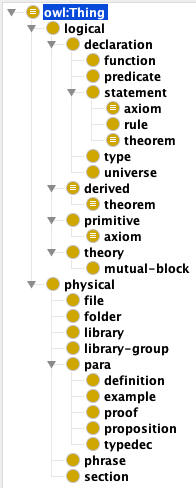
\includegraphics[width=3.5cm]{classes}\vspace*{-.5em}
  \caption{ULO Classes}\label{fig:classes}\vspace*{-3em}
\end{wrapfigure}
Note that while we hold the distinction of these five classes to be universal, concrete logics may not always distinguish them syntactically.
For example, HOL identifies functions and predicates, but the extractor can indicate whether a declaration's return type is the distinguished type of booleans.
Similarly, Curry-Howard-based systems identity predicates and types as well as statements and objects, which an extractor may choose to separate.

% The semantically meaningful sorts come in three pairs each containing a type-like sort $s$ and an object-like sort $t$.
% Intuitively, individuals $i$ and $j$ of sorts $s$ and $t$ occur together in some kind of is-a or is-instance-of relation such as a typing judgment $j:i$.


% \ind{type} and \ind{function}: These are the typical sorts of most objects.
%  In first-order logic, they correspond to sorts and function symbols.
%  In type theories, they correspond to type and function symbols.

%  FR: It's difficult to come up with good names for these. So I've introduced macros for now.
%  predicate used to be called 'proposition' but that is used elsewhere as a kind of theorem
%
%\truthType and \truthObject\ednote{these names are open for discussion, see source code}: In the Curry-Howard representation, these are special cases of \ind{type} and \ind{function}, but for relating and querying libraries, it is valuable to distinguish them, and even for systems that internally use the Curry-Howard representation, it is desirable to tease them apart.  $i$ is a \truthType if it is/returns a boolean, formula, judgment etc. (regardless of its truth value), and $i$ is a \truthObject if it is/returns anything that establishes the truth of such a formula (e.g.\ axiom, theorem, proof rule).
%
%We use the \ind{rule} class to indicate that a statement can be or is interpreted as a simplification or rewrite rule, Coq has more roles like these, e.g.: \ind{coercion} (to automatically cast a value from a type to another type), \ind{hint} (to automatically try to apply it when doing blind proof search), \ind{instance} of a type-class, to be used during user-guided proof search when guessing the parameters marked to be guessed using type-classes, \ind{morphism} to be used by setoid-rewriting tactics, etc.

Orthogonally to the above, we distinguish declarations by their definition status: \ind{primitive}{\isabelle\coq} if it introduces a new concept without a definition such as an urelement or an axiom; and \ind{derived}{\isabelle\coq} if it can be seen as an abbreviation for an existing concept like a defined operator or a theorem.
For example, intersecting the classes \truthObject and \ind{derived}, we capture all theorems.

While the primitive-derived distinction is clear-cut for definition-based systems like Coq, it is trickier for axiom-based systems like Isabelle: an Isabelle definition actually consists of a primitive concept with a defining axioms for it.
For that purpose, we introduce the \ind{defines} property in \S\ref{sec:objprops}.
%\ednote{CSC: possible alternative names: \ind{defined} and \ind{declared}. Question: is it worth distinguish between defined implicitly, e.g. as the unique object that has some property vs explicitly, by describing the object?}
  
\paragraph{Physical Role}
The physical classes describe an individual's role in the physical organization of a library.
This includes for an individual $i$:
\begin{compactitem}
 \item \ind{section}{\isabelle} if $i$ is an informal grouping inside a file (chapter, paragraph etc.)
 \item \ind{file}{\coq} if $i$ is a file
 \item \ind{folder}{\coq} if $i$ is a grouping level above source files inside a library, e.g., a folder, sub-package, namespace, or session
 \item \ind{library}{\coq} if $i$ is a library. Libraries have logical URIs and serve as the root objects containing all other individuals.
 A library is typically maintained and distributed as a whole, e.g., via a GitHub repository.
 A library has a logical URI and the URIs of individuals are typically formed relative to it.
 \item \ind{library-group}{\coq} if $i$ is a group of libraries, e.g., a GitHub group.
\end{compactitem}

\noindent In addition we define some classes for the lowest organizational level, called \emph{logical paragraphs}.
These are inspired by definition--example--theorem--proof seen in informal mathematics and often correspond to {\LaTeX} environments.
In formal libraries, the individuals of these classes may be the same as the ones for the logical classes or different ones.
For example, a document-oriented system like Isabelle could assign a physical identifier to a paragraph and a different logical one to the formal theorem inside it.
These identifiers could then have classes \ind{proposition} and \truthObject respectively. %\ednote{FR: This is a good example of our names still being unintuitive.}
A purely formal system could omit the physical class or add it to the logical identifier, e.g., to mark a logical definition as an \ind{example}{\coq} or \ind{counter-example}.
Some of these, in particular, theorems given informal classes like ``Lemma'' or ``Hauptsatz'', a string which can be specified by the \ind{paratype} relation (see below).
 
%We use the class \ind{phrase} for intra-sentential fragments of in mathematical text and formulae, these include symbols, declarations, and quantifications.

\subsubsection{Properties}\label{sec:objprops}

All properties are binary predicates whose first argument is an individual.
The second argument can be an individual (\textbf{object property}) or a value (\textbf{data property}).
Unless mentioned otherwise, we allow the same property to be used multiple times for the same individual.

The two kinds are often treated differently.
For example, for visualization as a graph, we can make individuals nodes (using different colors, shapes etc. depending on which classes a node has) and object properties edges (using different colors, shapes, etc. for different properties).
The data properties on the other hand would be collected into a key-value list and visualized at the node.
Another important difference is during querying: object properties are relations between individuals and thus admit relational algebra such as union and intersection or symmetric and transitive closure.
Data properties on the other hand are usually used with filters that select all individuals with certain value properties.

\paragraph{Library Structure}
Individuals naturally form a forest consisting e.g., of (from roots to leafs) library groups, libraries, folders, files, section, modules, groups of mutual recursive objects, constants.
Moreover, the dependency relation between individuals (in particular between the leaves of the forest) defines an orthogonal structure.

$\ind{specifies}(i,j)${\isabelle\coq} expresses that $j$ is a child of $i$ in the forest structure.
Thus, taking the transitive closure of \ind{specifies} starting with a library, yields all individuals declared in a library.

$\ind{uses}(i,j)${\isabelle\coq} expresses that $j$ was used to check $i$, where $j$ may include extra-logical individuals such as tactics, rules, notations.
A very frequent case is for $j$ to be an occurrence of a logical individual (e.g. a constant or a theorem). The case of occurrences leads to the question about what information can be attached to an occurrence. Examples could be: the number of repetitions of the occurrence; whether the occurrence of a constant induces a dependency on the type only, or on the actual definition as well; where the occurrence is located (e.g. in the statement vs proof, in the type vs body or in more specific positions, like as the head symbol of the conclusion, see~\cite{AGSTZ:ContMathSearchWhelp04} for a set of descriptions of positions that is useful for searching up to instantiation). For now we decided to avoid to specify occurrences in the ontology, for the lack of a clear understanding of what properties will really be useful for applications. Integrating the ULO ontology with occurrenes is left for future work towards ULO 1.0.

\paragraph{Semantic Relations between Declarations}
Relational representations treat individuals as black boxes.
But sometimes it is helpful to expose a little more detail about the internal structure of a declaration.
For that we define the following properties:
\begin{compactitem}
 \item $\ind{defines}(i,j)$ is used to relate a declaration $j$ to its definition $i$ if the two have different identifiers, e.g., because they occur in different places in the source file, or because $i$ is a defining axiom for a constant $j$.
 \item $\ind{justifies}(i,j)${\isabelle} relates any kind of argument $i$ to the thesis $j$ it supports. The most important example is relating a proof to its theorem statement if the two have different identifiers.
 \item $\ind{instance-of}(i,j)${\isabelle\coq} relates a structuring declaration $j$ to the theory-like entity $i$ that realizes, e.g., a module to its module type, an instance to its (type) class, a model to its theory, or an implementation to its specification.
 \item $\ind{generated-by}(i,j)$ expresses that $i$ was generated by $j$, e.g., the user may define an inductive type $j$ and the systems automatically generated an induction schema $i$.
 \item $\ind{inductive-on}(i,j)${\isabelle} expresses that $i$ is defined/proved by induction on the type $j$.
\end{compactitem}

\paragraph{Informal Cross-References}
First we define some self-explanatory cross-references that are typically (but not necessarily) used to link individuals within a library. These include \ind{same-as}, \ind{similar-to}, \ind{alternative-for}, \ind{see-also}, \ind{generalizes}, and \ind{antonym-of}.

Second we define some cross-references that are typically used to link a knowledge item in a library to the outside.
Of particular relevance are:
\begin{compactitem}
 \item $\ind{formalizes}(i,j)$ indicates that $j$ is an object in the informal realm, e.g., a theorem in an article, that is formalized/implemented by $i$.
 \item $\ind{aligned-with}(i,j)$ indicates that $i$ and $j$ formalize/implement the same mathematical concept (but possibly in different ways).
% \item \ind{inspired-by} and  are self-explanatory.
\end{compactitem}

\paragraph{Data Properties}
All properties so far were object properties.
Data properties are mostly used to attach metadata to an individual.
We do not introduce new names for the general-purpose metadata properties that have already been standardized in the Dublin Core such as
\verb|dcterms:creator|,
\verb|dcterms:title|,
\verb|dcterms:contributor|,
\verb|dcterms:description|,
\verb|dcterms:date|,
\verb|dcterms:isVersionOf|,
\verb|dcterms:source|,
\verb|dcterms:license|.
But we define some new data properties that are of particular interest for math libraries:
\begin{compactitem}
 \item $\ind{name}(i,v)${\isabelle\coq} attributes a string $v$ to a declaration that expresses the (user-provided) name as which it occurs in formulas.
 This is necessary in case an individual generated URI is very different from the name visible to users, e.g., if the URI is generated from an internal identifier or if the name uses characters that are illegal in URIs.
 \item $\ind{sourceref}(i,v)${\isabelle\coq} expresses that $v$ is the URI of the physical location (e.g., file, line, column in terms of UTF-8 or UTF-16 characters) of the source code that introduced $i$.
 \item $\ind{docref}(i,v)${\coq} expresses that $v$ is the URI reference to a place where $f$ is documented (usually in some read-only rich text format).
 \item $\ind{check-time}(i,v)${\isabelle} expresses that $v$ is the time (a natural number giving a time in milliseconds) it took to check the declaration that introduced $i$.
 \item $\ind{external-size}(i,v)${\isabelle} expresses that $v$ measures the source code of $i$ (similar to positions above).
 \item $\ind{internal-size}(i,v)${\coq} expresses that $v$ is the number of bytes in the internal representation of $i$ including inferred objects and generated proofs.
 \item $\ind{paratype}(i,v)${\isabelle} gives the ``type'' of a logical paragraph, i.e. something like ``Lemma'',  ``Conjecture'', \ldots. This is currently a string, but will become a finite enumeration eventually.
\end{compactitem}
Locations, sizes, and times may be approximate

\paragraph{Organizational Status}
Finally, we define a few (not mutually exclusive) classes that library management--related information such as being experimental or deprecated.
Many of these are known from software management in general.
The unary properties are realized as data properties, where the object is an explanatory string, the binary relations as object properties. 
An important logic-specific class is \ind{automatically-proved} --- it applies to any theorem, proof step, or similar that was discharged automatically (rather than by an interactive proof).

%%% Local Variables:
%%% mode: latex
%%% mode: visual-line
%%% fill-column: 5000
%%% TeX-master: "report"
%%% End:

%  LocalWords:  textbf organizational ednote swMATH irrelavant mathbb newcommand xspace mathrm emph formalized wrapfigure vspace includegraphics setoid-rewriting sec:objprops organization compactitem visualization visualized


\subsection{Exporting the Isabelle Knowledge Base}\label{sec:isabelle-export}
\subsubsection{Isabelle Overview}

Isabelle is a generic platform for tools based on formal logic.
It is generally known for its Isabelle/HOL library, which provides many theories and add-on tools (implemented in Isabelle/ML) in its \texttt{Main} theory and the \texttt{main} group of library sessions.
Some other (much smaller) Isabelle logics are FOL, LCF, ZF, CTT (an old version of Martin-L\"of Type Theory), but today most Isabelle applications are based on HOL.
The foundations of Isabelle due to Paulson~\cite{paulson700} are historically connected to \emph{logical frameworks} like Edinburgh LF: this fits nicely to the LF theory used in logic formalizations in MMT.
User contributions are centrally maintained in AFP, the \emph{Archive of Formal Proofs} (\url{https://www.isa-afp.org}).

From a high-level perspective, Isabelle is better understood as \emph{document-oriented proof assistant} or \emph{document preparation system} for domain-specific formal languages~\cite{Wenzel:IIdsflitd18}.
It allows flexible nesting of sub-languages, and types, terms, propositions, and proofs (in Isabelle/Isar) are merely a special case of that.
The result of processing Isabelle document sources consists of internal data structures in Isabelle/ML that are private to the language implementations.
Thus it is inherently difficult to observe Isabelle document content by external tools, e.g.\ to see which $\lambda$-terms occur in nested sub-languages.

Isabelle/PIDE \cite{Wenzel:2014:ITP-PIDE}, the Prover IDE framework, integrates all
activities of development for proofs and programs into a
\emph{semantic editor} Isabelle/jEdit. While the user is composing
text, the prover provides real-time feedback about its meaning: that
rich PIDE markup information can be rendered as conventional GUI
metaphors (e.g.\ text color, squiggly underline, tooltips, hyperlinks,
icons in the border) \cite{Wenzel:2019:MKM}. It is also possible to
run Isabelle/PIDE in ``headless mode'', to let some Isabelle/Scala
program observe markup as a formal library is processed in
Isabelle/ML.

The standard distribution of Isabelle\footnote{\url{https://isabelle.in.tum.de}} includes the
Isabelle/HOL library with various applications, but the main bulk of
applications is in the \emph{Archive of Formal Proofs}
(AFP)\footnote{\url{https://www.isa-afp.org}}, which is organized like
a scientific online journal. In August 2019, Isabelle/AFP had 492
articles by 331 authors, comprising 120\,MB source text total. Formal
checking requires approx.\ 50h CPU time or 2h elapsed time on high-end
multicore hardware. The result is a collection of heap images for the
internal state of Isabelle/ML and some HTML or PDF documents that
resemble conventional mathematical texts (with relatively little
formal markup being used here).


% % % % % % % % % % % % % % % % % % % % % % % % % % % % % % % % % % % % % % % % % % % % % % % % % % %
\subsubsection{General Technical Aspects of Exporting Isabelle Knowledge Bases}

Isabelle/ML is the \emph{internal implementation language} for logic-based tools, has direct access to the inference kernel in the manner of the ``LCF-approach'' \cite{Gordon-Milner-Wadsworth:1979}.
Isabelle/Scala is the \emph{external interface language} to manage Isabelle processes and
resulting content: it has access to the physical world with GUI frameworks, TCP servers, database engines etc.

To support exports like ours systematically, Wenzel had previously already instrumented the theory processing in Isabelle/ML to allow arbitrary \emph{presentation} for every theory node as it is finished: an ML function gets access to all commands with their intermediate theory
values; it can extract suitable information and \emph{export} it via a private channel to Isabelle/Scala.
The standard configuration of Isabelle provides options like \verb,export_theory, or \verb,export_proofs, to externalize certain aspects of theory content as a \emph{session database}.
For example, see command-line tools like \verb,isabelle build -o export_theory HOL-Analysis, to build such a database (for SQLite) and \verb,isabelle export -l HOL-Analysis, to query it later on.

Isabelle/Scala provides direct access to session builds and their results as an API for \emph{typed functional-object-oriented programming}: this is more robust and versatile than command-line tools.
For our export, we use the Isabelle/Scala APIs to provide dedicate command-line \verb,isabelle mmt_import,: options and arguments similar to \verb,isabelle build, specify a collection of sessions to be processed, the results are given to the MMT Scala API to write files in OMDoc format; there is extra output of RDF/XML files.

Our export (Isabelle repository version e6fa4b852bf9) turns this content into OMDoc and RDF/XML.
Our command-line tool uses regular Scala APIs of MMT (without intermediate files), and results are written to the file-system in OMDoc and RDF/XML format.
It runs a Prover IDE session (PIDE) under program control: a collection of \emph{sessions} with corresponding \emph{theories} is turned into formal source edits that are given to Isabelle/PIDE for semantic processing; the underlying prover process continuously produces markup reports as it explores the meaning of the source.
Whenever some theory node (with all imports) is finished, a separate Scala operation is invoked to \emph{commit} the result as
PIDE \emph{document snapshot}.
Thus the application can harvest theory exports produced up to that point, and the system can edit-out already processed theory-subgraphs to free resources, while the overall process is still running.

Thus the full material of AFP (hundreds of sessions, thousands of theories) can be digested on a high-end multicore machine within
approx. 24h elapsed time using 60 GB RAM for Isabelle/ML and 30 GB RAM for Isabelle/Scala.
This is approximately a factor 10 more than a conventional batch build, but the PIDE session is able to ``see'' more detailed information about the formal meaning of the sources (e.g.\ the use of term constants within the theory text, like the IDE front-end uses to provide hyperlink operations).

% % % % % % % % % % % % % % % % % % % % % % % % % % % % % % % % % % % % % % % % % % % % % % % % % % %
\subsubsection{Exporting Symbolic Knowledge in OMDoc/MMT Format}

We export all \emph{logical foundations} of theory documents (types, consts, facts, but \emph{not} proof terms), and aspects of \emph{structured specifications} (or ``little theories'') (locales and locale interpretations, which also subsumes the logical content of type classes).
Figure~\ref{fig:isabellemmt} shows a screenshot of the MMT browser showing a small part (the definition of binomial coefficients in Isabelle/HOL) of the exported Isabelle knowledge base.

\begin{figure}[ht]
  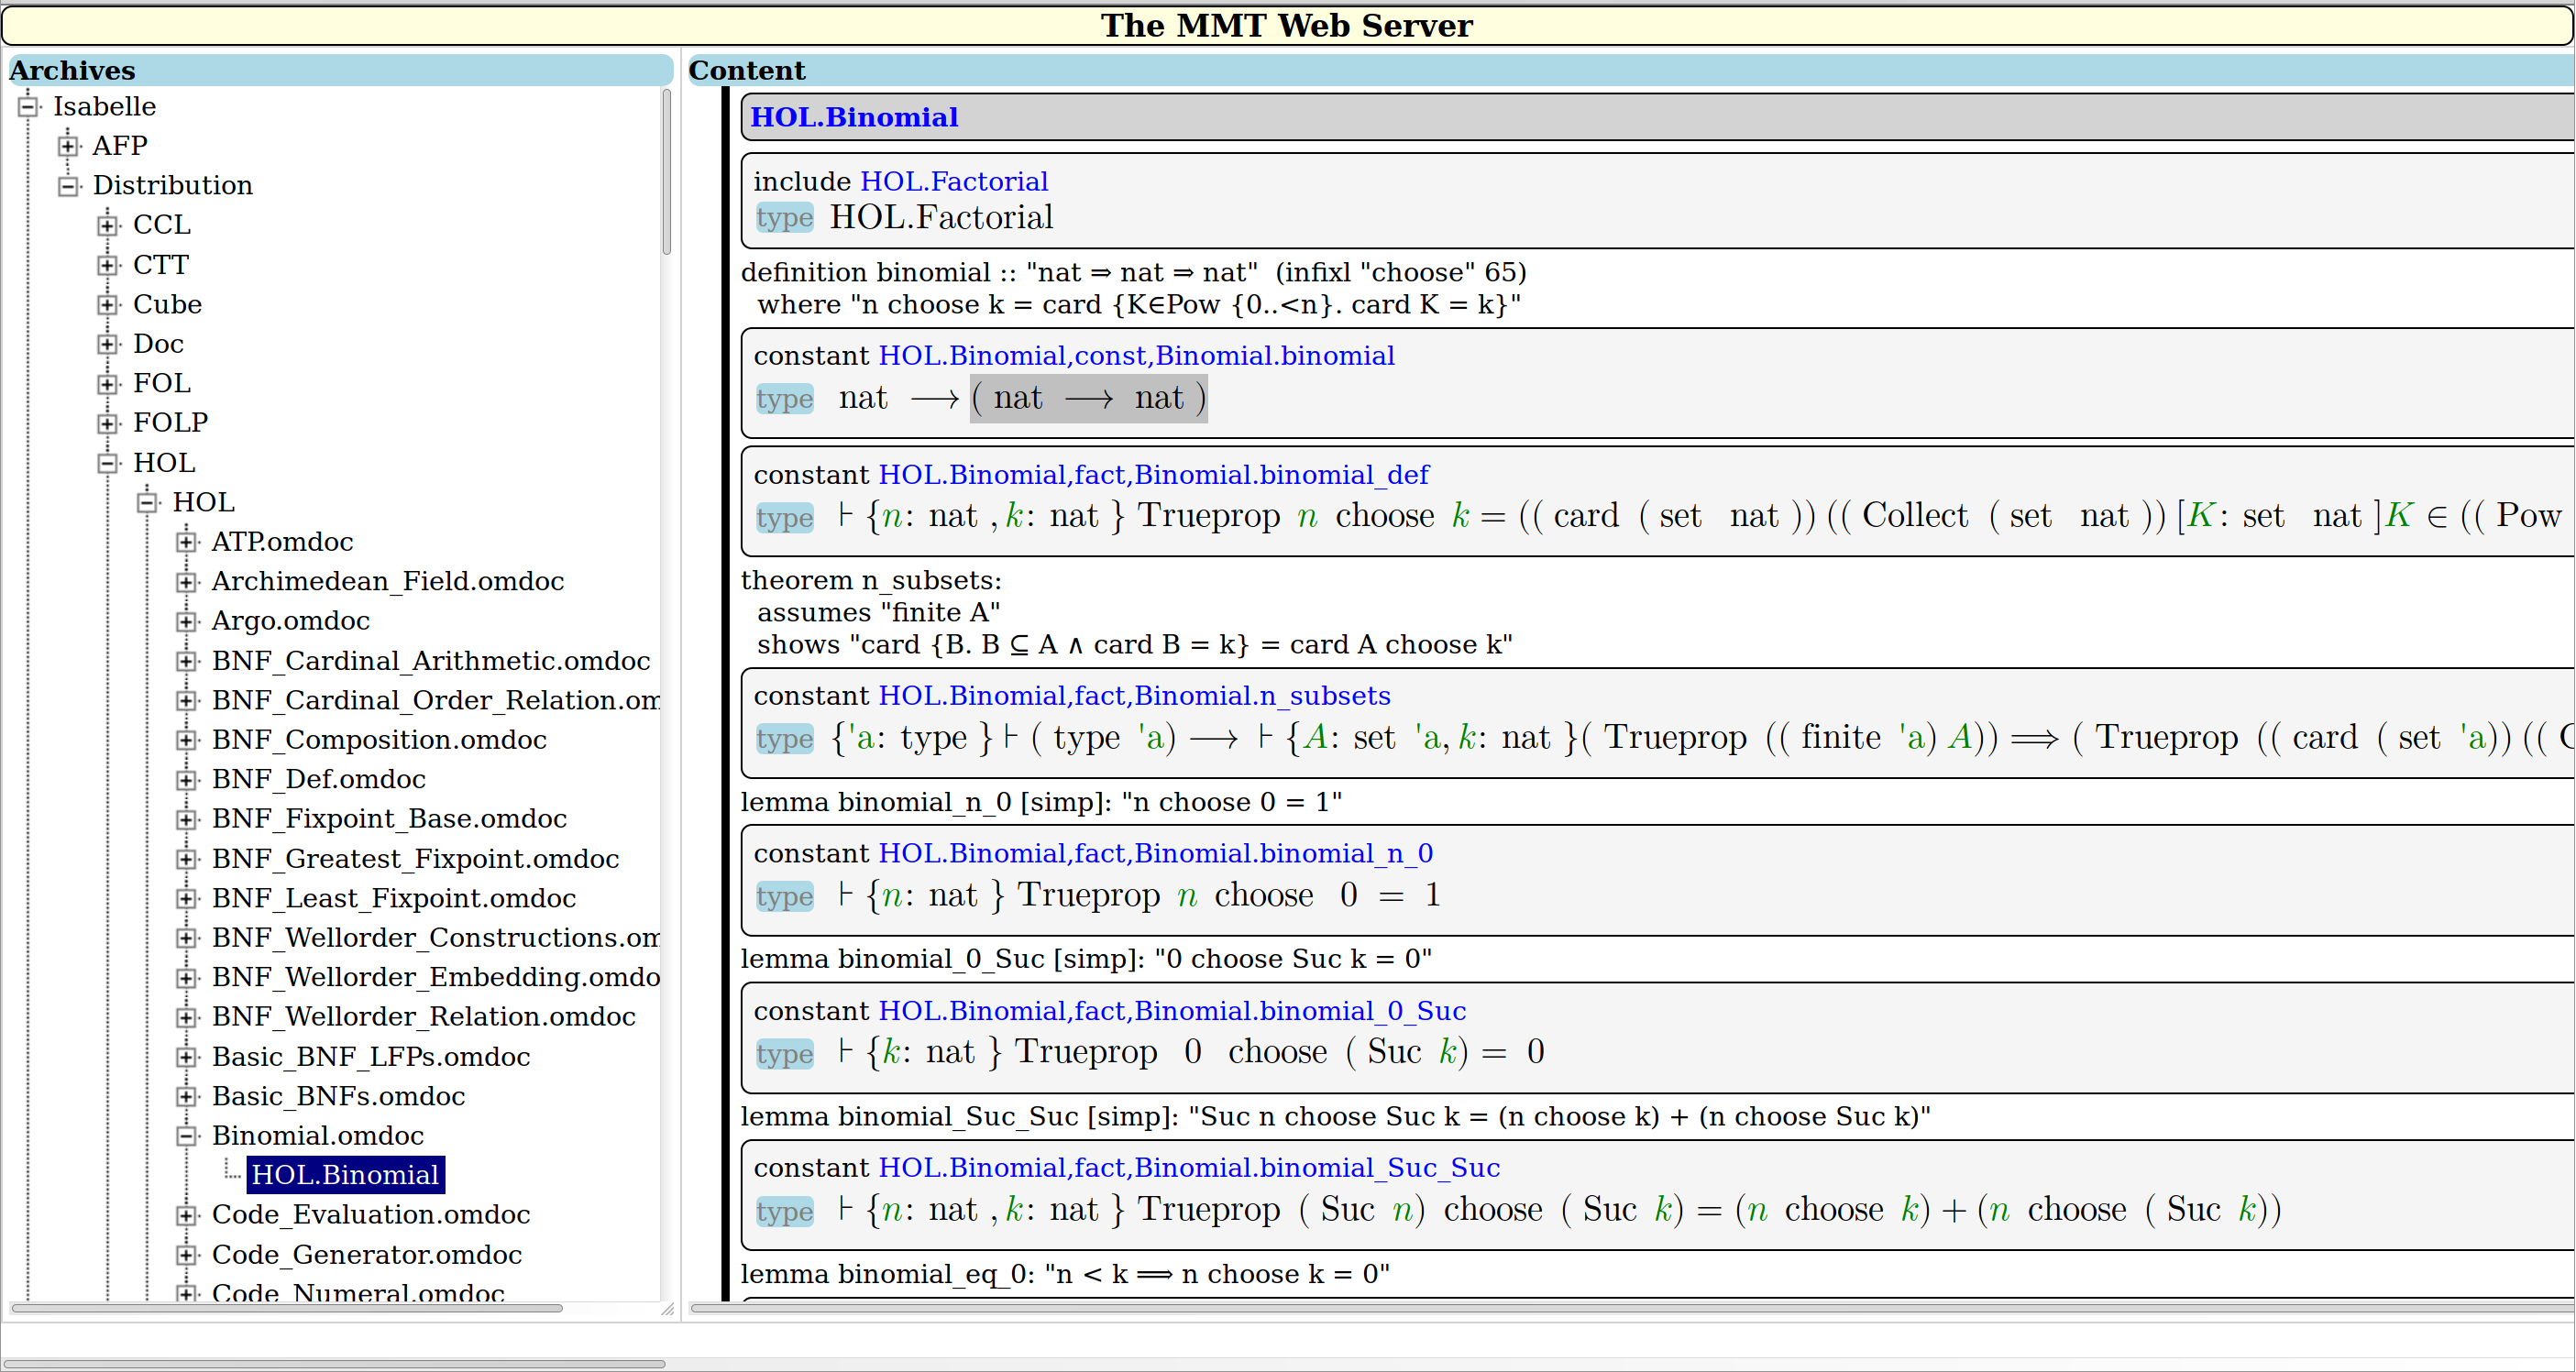
\includegraphics[width=\textwidth]{isabelle_mmt}
  \caption{MMT browser showing Isabelle content}\label{fig:isabellemmt}
\end{figure}

\paragraph{Module System}
All module system--level Isabelle entities are represented as MMT theories and morphisms.
These use a manually written MMT meta-theory that formalizes Isabelle/Pure --- the logic underlying Isabelle.

Besides plain Isabelle theories, this includes the order-sorted algebra of \emph{type classes} (subclass relation) and \emph{type arities} (image behavior of type constructors wrt.\ type class domains and ranges) in the sense of Nipkow and Prehofer \cite{Nipkow-Prehofer:1993} as well as locales in the sense of Ballarin \cite{Ballarin2014} and type classes as special locale interpretations in the sense of Haftmann and Wenzel \cite{Haftmann-Wenzel:2006:classes,Haftmann-Wenzel:2009}.

  Isabelle locales are \emph{named contexts} with type parameters
  (implicit), term parameters (\textbf{fixes}), and premises
  (\textbf{assumes}). Within such a ``little theory'' it is possible
  to spell out definitions, statements, proofs as usual --- all
  results are understood as relative to the context. The foundations
  will contain an extra prefix of type variables, term abstractions
  and assumptions according to the context.

  The export of locales preserves some of its internal structure,
  notably the locale dependency relation stemming from the
  construction of locales and sub-locales (by definition), as well as
  later locale interpretations (by proof).

  Type classes are special locales with a single type parameter and a
  canonical locale interpretation to connect \emph{type class
    parameters} (polymorphic constants with class constraints) to
  \emph{locale parameters} (fixed variables of the context). The
  export shows the result of the interpretation, but \emph{without} an
  explicit report on their connection.


\paragraph{Declarations}
Every declaration in a theory-like scope is represented as an MMT declaration.
This includes \textbf{types} (base types and type constructors),
  term \textbf{constants} (including functions, binders, quantifiers
  as higher-order constants), \textbf{axioms} (including equational
  axioms that count as primitive definitions), and \textbf{theorems}
  (propositions with a proof).

Isabelle definitions become equational axioms in MMT.
This includes theorems, which are treated as defined constants in MMT via the Curry-Howard representation.
However, the actual proofs, which become the definientia of these constants, are not exported by default (proof terms are prohibitively large), but it is possible to reconstruct the source text in the Isabelle/Isar proof language from the position information.

Type definitions in the sense of Gordon and
  Pitts \cite{pitts93} are interpreted
  definitionally within the standard semantics of the HOL
  logic. The export facility provides access to the key
  information: the old representing type, the new abstract type, the
  name of the morphisms between the two with the axiom stating the
  relation.
  This information allows recovering HOL typedefs faithfully, where
  Isabelle/Pure theory content would only show the individual
  particles. It also serves as an example to ``query'' derived
  specification mechanisms in Isabelle/ML, to expose its own level of
  abstraction to the exporter.
  
Term constants with indication of derived specifications
  mechanisms, e.g.\ \textbf{primrec} functions, \textbf{inductive} or
  \textbf{coinductive} relations are handled by querying generic
  information in Isabelle/Pure about functional or relation
  specifications (so-called ``Spec Rules''). The Isabelle/HOL
  implementations provide this data on their own account.

\paragraph{Expressions}
The expressions of Isabelle's $\lambda$-calculus are represented as MMT terms.
This part of the translation is relatively straightforward and similar to previous exports to OMDoc/MMT (e.g., \cite{KalRab:hollight:14,KohMueOwr:mpagsiuf17,MueRabSac:cltg19}).
Only the treatment of variables warrants further description, and we focus on it in the sequel.

Isabelle variables come in various flavours: free variables (e.g.\
\verb,x,), schematic variables with index (e.g. \verb,?x10,) and bound
variables (e.g. \verb,x, in $\lambda$\verb,x::,$\tau$\verb,. x, which
is concrete syntax for the de-Bruijn index abstraction
\verb;Abs (x, ;$\tau$\verb;, B.0); where \verb,x, is retained as a
comment). To fit smoothly into the lambda-calculus of MMT, variable
names are standardized as follows:

Schematic variables are renamed to fresh free variables. Since
  schematic variables are morally like a universal quantifier prefix,
  this preserves the logical meaning of a formala (e.g.\ a theorem
  statement).

Bound variable comments in abstractions are renamed locally to
  avoid clashes with free variables in the same scope. Thus the
  comment can be used literally in MMT/LF as named abstraction,
  ignoring the unnamed de-Bruijn index representation of Isabelle.

Finally, Isabelle type variables are decorated with type class constraints,
e.g.\ \verb,'a::order, for types that belong to the class \verb,order,
defined in the Isabelle/HOL library (e.g.\ \verb,nat, with its
standard order): this ensures certain \emph{operations} with a link to
overloaded term constants (e.g.\ \verb,less :: 'a => 'a => bool,), as
well as logical \emph{premises} on these operations (e.g.\ stating
that \verb,less, is a strict order on the type).

Isabelle class operations are managed by extra-logical means, e.g.\ by
the code-generator for Haskell or Standard ML, to produce the expected
\emph{dictionary construction} to eliminate the implicit
overloading. In MMT this will merely result in uncontrolled
polymorphism: constant definitions consist of multiple
(non-overlapping) equational specifications depending on the type
argument.

Isabelle class premises become logical constraints in a
straight-forward manner: a type class is a predicate over types in LF,
so \verb,'a::c, means that the predicate \verb,c, applied to type
\verb,'a, holds. Statements with class constraints
$\phi($\verb,'a::c,$)$ are augmented by a prefix of preconditions
\verb,'a::c,${} \Longrightarrow \phi($\verb,'a,$)$, effectively
eliminating the constraint within the logic.

\paragraph{Identifiers}
Isabelle constants live in separate name spaces (for types, terms,
theorems etc.).  For example, there could be a type \verb,Nat.nat, and
a term constant of the same name (e.g.\ an operation to make a natural
number). Qualification is usually by the theory \emph{base} name, not
the session-qualified long name; in rare situations, there is no
theory qualification at all. In order to have all entities coexist
within one big space of individuals in MMT, we use a triple that
consists of (\emph{long-theory-name}, \emph{entity-name},
\emph{entity-kind}) written as URI like as follows:

\begin{quote}
\texttt{https://isabelle.in.tum.de?}\emph{long-theory-name}\texttt{?}\emph{entity-name}\texttt{|}\emph{entity-kind}
\end{quote}

\noindent For example, \texttt{https://isabelle.in.tum.de?HOL.Nat?Nat.nat|type} refers to the type of natural numbers in the Isabelle/HOL library.


% % % % % % % % % % % % % % % % % % % % % % % % % % % % % % % % % % % % % % % % % % % % % % % % % % %
\subsubsection{Exporting Relational Knowledge in ULO Format}

Relations between formal items are output as RDF/XML triples,
  bypassing MMT and its OMDoc format; see also
  \cite[\S3.1]{ConKohMue:rdaml19}.  This also captures some aspects of
  inductive and primitive recursive definitions via
  \verb,ulo:inductive-on,. In addition to that paper, there is now
  full coverage of theorem dependencies via \verb,ulo:uses,, spanning
  a rather large dependency graph over the source text: it relates
  theorem statements with used constants and proofs with used
  theorems.  



\paragraph{Individuals}
Formal entities are identified by their \emph{name} and \emph{kind} as follows:
\begin{compactitem}
\item The name is a long identifier (with dot as separator, e.g.\ \texttt{Nat.Suc}) that is unique within the current theory context (including the union of all theory imports). Long names are managed by namespaces within the formal context to allow partially qualified names in user input and output (e.g.\ \texttt{Suc}). The structure of namespaces is known to the prover, and not exported.
\item The kind is a short identifier to distinguish the namespaces of formal entities, e.g.\ \texttt{type} for type constructors, \texttt{const} for term constants, \texttt{fact} for lists of theorems that are recorded in the context, but also non-logical items like \texttt{method} (Isar proof methods), \texttt{attribute} (Isar hint language) etc.
\end{compactitem}

\noindent
This name/kind scheme is in contrast to usual practice in universal $\lambda$-calculus representations like MMT/LF, e.g.\ there could be a type \texttt{Nat.nat} and a separate term constant of the same name.  Moreover the qualification in long names only uses theory base names, not their session-qualified long name (which was newly introduced in Isabelle2017). So in order to support one big space of individuals over all Isabelle sessions and theories, we use the URI format that was already used for identifiers above.

\paragraph{Logic}
The primitive logical entities of Isabelle/Pure are types, terms, and theorems (facts).
Additionally, Isabelle supports various theory-like structures.
These correspond our declaration classes as follows:
\begin{compactitem}
\item \ind{theory} refers to global \textbf{theory} and local \textbf{locale} contexts. There are various derivatives of \textbf{locale} that are not specifically classified, notably \textbf{class} (type classes) and \textbf{experiment} (locales with inaccessible namespace).
\item \ind{type} refers to \emph{type constructors} of Isabelle/Pure, and object-logic types of many-sorted FOL or simply-typed HOL. These types are syntactic, and not to be confused with the ``propositions-as-types'' approach in systems like Coq. Dependent types are represented as terms in Isabelle.
\item \ind{function} refers to \emph{term constants}, which are ubiquitous in object-logics and applications. This covers a broad range of formal concepts, e.g.\ logical connectives, quantifiers (as operators on suitable $\lambda$-terms), genuine constants or mathematical functions, but also recursion schemes, or summation, limit, integration operators as higher-order functions.
\item \ind{statement} refers to individual theorems, which are projections from the simultaneous \texttt{fact} lists of Isabelle.  Only the head statement of a theorem is considered, its proof body remains abstract (as reference Isar to proof text).
Theorems that emerge axiomatically (command \textbf{axiomatization}) are marked as \ind{primitive}, properly proven theorems as \ind{derived}, and theorems with unfinished proofs (command \textbf{sorry}) as \ind{experimental}.
\end{compactitem}

\noindent The \ind{specifies} and \ind{specified-in} relations connect theories and locales with their declared individuals.
The \ind{uses} relation between those represents syntactic occurrence of individuals in the type (or defining term) of formal entities in Isabelle: it spans a large acyclic graph of dependencies. Again, this excludes proofs: in principle there could be a record of individuals used in the proof text or by the inference engine, but this is presently unimplemented.

The \ind{source-ref} property refers to the defining position of formal entities in the source.
Thanks to Isabelle/PIDE, this information is always available and accurate: the Prover IDE uses it for highlighting and hyperlinks in the editor view. Here we use existing URI notation of MMT, e.g.\ \url{https://isabelle.in.tum.de/source/FOL/FOL/FOL.theory#375.19.2:383.19.10} with offset~/ line~/ column of the two end-points of a text interval.

The \ind{check-time} and \ind{external-size} properties provide some measures of big theories in time (elapsed) and space (sources).  This is also available for individual commands, but it is hard to relate to resulting formal entities: a single command may produce multiple types, consts, and facts simultaneously.

\paragraph{Semi-formal Documents}
We use \ind{section} for the six levels of headings in Isabelle documents: \textbf{chapter}, \textbf{section}, \dots, \textbf{subparagraph}.  These are turned into dummy individuals (which are counted consecutively for each theory).

\ind{file}, \ind{folder}, \ind{library} are presently unused.
They could refer to the overall project structure Isabelle document sources in the sense of~\cite{Wenzel:IIdsflitd18}, namely as \emph{theories} (text files), \emph{sessions} (managed collections of theories), and \emph{project directories} (repository with multiple session roots).

For document metadata, we use the Dublin Core ontology.  The Isabelle command language has been changed to support a new variant of \emph{formal comment}. With one keystroke, the presentation context of a command may be augmented by arbitrary user-defined marker expressions. Isabelle/Pure already provides \texttt{title}, \texttt{creator}, \texttt{contributor} etc.\ from \S\ref{sec:objprops}: they produce PIDE document markup that Isabelle/MMT can access and output as corresponding RDF.

This approach allows to annotate theory content \emph{manually}: a few theories of \texttt{HOL-Algebra} already use the new feature sporadically. For automatic marking, metadata of AFP entries is re-used for their theories. One could also digest comments in theory files about authors, but this is presently unimplemented.


\subsubsection{Statistics}\label{sec:stats}

We present some statistics\footnote{Versions: Isabelle/9c60fcfdf495, AFP/d50417d0ae64, MMT/e6fa4b852bf9.}.
This gives an idea about overall size and scalability of the export facilities so far.
The datasets are publicly available from \url{https://gl.mathhub.info/Isabelle}.

{\tiny
\begin{center}
\begin{tabular}{cl||r|r||r|r|r|r|r||r|r}
  & Library                       & Individuals & Relations  & Theories & Locales  & Types      & Constants & Statements  & RDF/XML    & elapsed \\
  &                               &             &            &          &          &            &           &             & file size  & time \\\hline
  \isabelle & Distribution        &     103,873 &  2,310,704 &      535 &     496  &   235      & 8,973     &     88,960  & 188\,MB    & 0.5h \\
            & only group                                                                                                    
                    \texttt{main} &             &            &          &          &            &           &             &            & \\\hline
  \isabelle & Distribution+AFP    &   1,619,889 & 36,976,562 &    6,185 &  4,599   & 10,592     & 215,878   &  1,359,297  & 3,154\,MB  & 16.5h \\
            & without \verb,very_slow,
                                  &             &            &          &          &            &           &             &            & \\\hline
%  \coq      & All 49 Libraries    & 383,527     & 11,516,180 &    1,979 & -        &  6,061     & -         &  161,736    & 452\,MB    & \\
\end{tabular}
\end{center}}

%%% Local Variables:
%%% mode: latex
%%% mode: visual-line
%%% fill-column: 5000
%%% TeX-master: "report"
%%% End:

%  LocalWords:  subsubsection texttt texttt paulson700 emph Wenzel:IIdsflitd18 organized verb,export_theory verb,export_proofs externalize verb,isabelle verb,isabelle consts fig:isabellemmt includegraphics textwidth isabelle_mmt arities wrt Prehofer Nipkow-Prehofer:1993 Ballarin Ballarin2014 textbf pitts93 primrec coinductive ednote pvs verb,x verb,order verb,nat verb,less verb,c Longrightarrow noindent ConKohMue:rdaml19 verb,ulo:inductive-on verb,ulo:uses compactitem axiomatization sec:objprops hline verb,very_slow


\subsection{Applications}\label{sec:uloappl}
% \ednote{FR: Picking 1 of the 3 queries given here is enough as an example.
% The paragraph 'Additional Examples' should be removed, and 1-2 of the difficult queries given there should be given as advanced examples.
% Try to give one screenshot of the result of a complex query. Say how many results the queries return.}

In this section, we evaluate the ULO framework, i.e. the ULO ontology and the generated RDF data by showing how they could be exploited using standard tools of the Semantic Web tool stack.

We have set up an instance of Virtuoso Open-Source Edition\footnote{\url{https://github.com/openlink/virtuoso-opensource}}, which reads the exports described in Section~\ref{sec:isabelle-export} and provides a web interface with a SPARQL endpoint to experiment with the ULO dataset.
Then we have tried several queries with promising results (just one shown below for lack of space).
The queries are not meant to be a scientific contribution per se: they just show how much can be accomplished with the ULO dataset with standard tools in one afternoon.

\paragraph{Example query: all recursive functions on $\mathbb{N}$} For this, we use the \lstinline|ulo:inductive-on| relation to determine inductive definitions on a type \lstinline|?y|, which we restrict to one that is aligned with the type \lstinline|nat_lit| of natural numbers from the interface theory \lstinline|NatLiterals| in the Math-in-the-Middle Ontology.
\begin{lstlisting}
SELECT ?x ?y WHERE {
  ?x ulo:inductive-on ?y .
  http://mathhub.info/MitM/Foundation?NatLiterals?nat_lit ulo:aligned-with ?y . }
\end{lstlisting}
Note that we use alignments~\cite{MueGauKal:cacfms17} with concepts from an interface theory as a way of specifying ``the natural numbers'' across theorem prover libraries. The result is a list of pairs: each pair combines a specific implementation of natural numbers (Isabelle has several, depending on the object-logic), together with a function defined by reduction on it. A subset of the results of this query are shown in Figure~\ref{fig:query}.

\begin{figure}[t]\centering
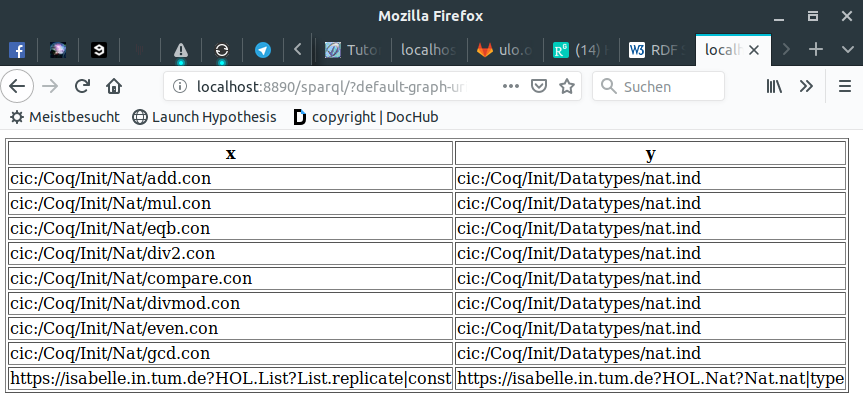
\includegraphics[width=\textwidth]{ulo_queryresult}
\caption{Virtuoso Output for the Example Query using Alignments}\label{fig:query}
\end{figure}

\ednote{check if Dennis can supply Isabelle screenshots}

%Similarly,  we can e.g. use the \lstinline|ulo:orcid| and \lstinline|dcterms:creator| properties to e.g. query for all theorems by Michael Kohlhase or Claudio Sacerdoti Coen using their ORCID.

\paragraph{Transitive Queries} The result of the query above only depends on the explicitly generated RDF triples. Semantic Web tools that understand OWL allow more complex queries. % For example, if we want to query for \emph{all theorems whose proofs depend on statements with incomplete proofs}, it is sufficient to specify in the ontology that \ind{uses} is transitive, and add a property to identify incomplete proofs.
For example, Virtuoso implements custom extensions that allow for querying the transitive closure of a relation. The resulting query syntax is a little convoluted, and we omit some details in the example below.
\begin{lstlisting}
SELECT ?o ?dist WHERE { {
      SELECT ?s ?o WHERE { ?s ulo:declares ?o }
    }
    OPTION ( TRANSITIVE, t_distinct, t_in(?s), t_out(?o), t_min (1),
             t_max (10), t_step ('step_no') as ?dist ) .
    FILTER ( ?s = <https://isabelle.in.tum.de?HOL.Nat> )
  }
ORDER BY ?dist DESC 2
\end{lstlisting}
The above code queries for all symbols recursively declared in the (effectively randomly chosen) Theory \texttt{HOL.Nat} declaring the natural numbers and associated concepts; the output for that query is shown in Figure \ref{fig:query2}.


\begin{figure}[ht]\centering
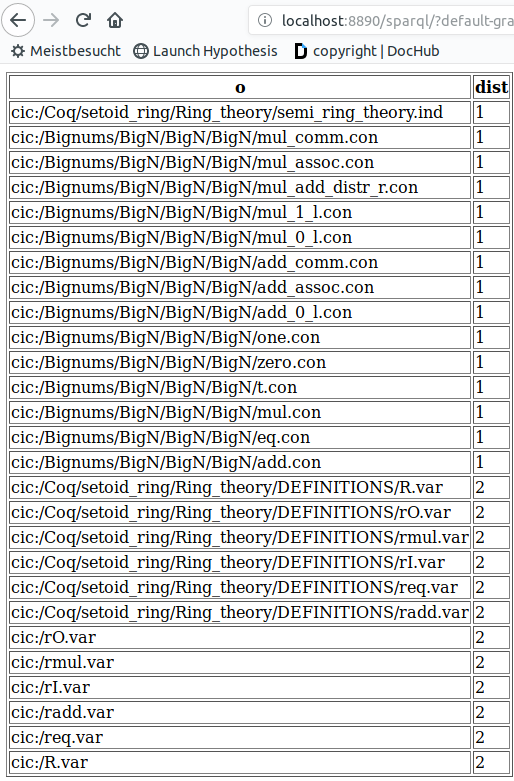
\includegraphics[width=0.5\textwidth]{ulo_queryresult2}
\caption{Virtuoso Output for the Transitive Example Query}\label{fig:query2}
\end{figure}

%then we have to use that the \ind{ulo:uses} is transitive.
%This is specified in the OLW2 implementation ULO ontology and can be used by sufficiently powerful tools (e.g. Virtuoso).
%Given that Virtuoso implicitly computes the transtive closure we can answer the query using a very similar query as the one above (given an alignment for proof gap objects).

Interesting examples of library management queries which can be modeled in SPARQL (and its various extensions, e.g. by rules) are found in~\cite{conf/lpar/AspinallDL12}. Instead~\cite{AGSTZ:ContMathSearchWhelp04,MKM04:AspertiS04} show examples of interesting queries (approximate search of formulae up to instantiation or generalization) that can be implemented over RDF triples, but that requires an extension of SPARQL with subset and superset predicates over sets.
% \ednote{DM: Add detailed examples (transitivity?)}
%\begin{center}
%\begin{tabular}{|c|c|}\hline
%	\lstinline|x| & \lstinline|y| \\\hline\hline
%	\tiny\lstinline>https://isabelle.in.tum.de?HOL.List?List.replicate|const> & \tiny\lstinline>https://isabelle.in.tum.de?HOL.Nat?Nat.nat|type> \\\hline
%	\tiny\lstinline|cic:/Coq/Init/Nat/add.con| & \tiny\lstinline|cic:/Coq/Init/Datatypes/nat.ind| \\\hline
%	\tiny\lstinline|cic:/Coq/Init/Nat/mul.con| & \tiny\lstinline|cic:/Coq/Init/Datatypes/nat.ind| \\\hline
%	\tiny\lstinline|cic:/Coq/Init/Nat/div2.con| & \tiny\lstinline|cic:/Coq/Init/Datatypes/nat.ind| \\\hline
%\end{tabular}
%\end{center}
%
%\paragraph{All theorems by Michael Kohlhase or Claudio Sacerdoti Coen}\ 
%\begin{lstlisting}
%SELECT ?x WHERE {
% ?x [ulo:theorem ?y ; dcterms:creator ?z]
% {?z ulo:orcid "0000-0002-4360-6016"} 
%   UNION
% {?z ulo:orcid "0000-0002-9859-6337"} }
%\end{lstlisting}
%
%\paragraph{All theorems with incomplete Proofs}\
%\begin{lstlisting}
%SELECT ?x WHERE {
%  ?x [ulo:proof ?y ; ulo:uses ?z]
%  ?z ulo:aligned-with http://mathhub.info/MitM?proofs?gap
%  OPTION ( TRANSITIVE, t_distinct, t_in(?x),t_out(?z)) }
%\end{lstlisting}
%This query is similar to the one about all inductive functions above, only that we use transitivity for the \lstinline|ulo:uses| relation (SPARQL syntax simplified).\ednote{MK: I have copied this by pattern matching from \url{https://virtuoso.openlinksw.com/tutorials/sparql/SPARQL_Tutorials_Part_5/SPARQL_Tutorials_Part_5.html} without understanding much.\\DM: Doing this properly gets ugly and elaborate; I would leave it simplified.}
%
%\paragraph{Additional examples} include
%\begin{itemize}
%\item Authors with the slowest proofs (in verification)
%\item Libraries ordered by dependency and check-time
%\item Dependency paths by cumulative check time
%\item Subgraphs by Topology; e.g. all situations of the form
%  \begin{tikzpicture}[baseline=(c.base),xscale=1.4,yscale=.8]
%    \node (lo) at (0,1) {$\bullet$};
%    \node (ro) at (1,1) {$\bullet$};
%    \node (lu) at (0,0) {$\bullet$};
%    \node (ru) at (1,0) {$\bullet$};
%    \node (c) at (.5,.5){};
%    \draw[include] (lu) -- (lo) ;
%    \draw[include] (ru) -- (ro);
%    \draw[struct] (lo) -- node[above]{\tiny deps} (ro);
%  \end{tikzpicture}
%  in a given library.
%\end{itemize}
%%% Local Variables:
%%% mode: latex
%%% mode: visual-line
%%% fill-column: 5000
%%% TeX-master: "report"
%%% End:

%  LocalWords:  ednote mathbb MueGauKal:cacfms17 centering includegraphics textwidth queryresult emph hline texttt BigNring AGSTZ:ContMathSearchWhelp04,MKM04:AspertiS04 generalization


%%% Local Variables:
%%% mode: latex
%%% mode: visual-line
%%% fill-column: 5000
%%% TeX-master: "report"
%%% End:

%  LocalWords:  ednote sec:uloappl mathbb Makarius optimized sec:appl ulo_appl RabKoh:WSMSML13,DehKohKon:iop16,KohMuePfe:kbimss17 taskref dksbases MueRabSac:cltg19


\newpage
\section{Mathematical Datasets}\label{sec:data}
\paragraph{Mathematical Datasets}
% Innovations based on mathematical knowledge and algorithms yield many improvements in science, engineering, economy, ecology, health care, security, and society overall. 
% For example, our global positioning system (GPS) needs the mathematics of relativistic physics, our mobile phones use frequencies allocated through combinatorial optimization, the combinatorics of our genome yields clues to curing rare diseases, the privacy of our communications depends on cryptographic protocols steeped in number theory, and our national security is relying on the mathematical analysis of increasingly complex networks. 
% Fundamental mathematical research and its direct application in practical situations enable many engineering, science, and business innovations that enrich society and mankind.\ednote{FR: throw out this paragraph? Or replace with one sentence?}

Modern mathematical research increasingly depends on collaborative tools, computational environments, and online databases, and these are changing the way mathematical research is conducted and how it is turned into applications.
For example, engineers now use mathematical tools to build and simulate physical models based on systems of differential equations with millions of variables, combining building blocks and algorithms taken from libraries shared all over the internet.

Traditionally, mathematics has not paid particular attention to the creation and sharing of data --- the careful computation and publication of logarithm tables is a typical example of the extent and method.
This has changed with the advent of computer-supported mathematics, and the practice of modern mathematics is increasingly data-driven.
Today it is routine to use mathematical datasets in the Gigabyte range, including both human-curated and machine-produced data.
Examples include the L-Functions and Modular Forms Database (LMFDB; $\sim 1$ TB data in number theory)~\cite{Cremona:LMFDB16,lmfdb:on} and the GAP Small Groups Library~\cite{GapSmallGroups:on} with $\sim 450$ million finite groups.  
In a few, but increasingly many areas, mathematics has even acquired traits of experimental sciences in that mathematical reality is ``measured'' at large scale by running computations.

There is wide agreement in mathematics that these datasets should be a common resource and be open and freely available.
Moreover, the software used to produce them is usually open source and free as well.
%While FAIR does not necessarily mean Open~\cite[2.3]{FAIR}, the appropriate Openness for almost all mathematical data is indeed open source and free.
Such an ecosystem is embraced by the mathematics community as a general vision for their future research infrastructure~\cite{NAS14}, adopted by the International Mathematical Union as the Global Digital Mathematics Library initiative \cite{GDML:on}.

To better understand the scale of the problem, Figure~\ref{fig:datasets} gives an overview over some state-of-the-art datasets.
Here we already use the division into four kinds of mathematical data that we will develop in Section~\ref{sec:fair}.

\paragraph{State of FAIRness for Mathematical Datasets}
Mathematical datasets are generally produced, published, and maintained with virtually no systematic attention to the FAIR principles~\cite{FAIR,WilDumAal:FAIR16} for making data findable, accessible, interoperable, and reusable.
In fact, often the sharing of data is an afterthought --- see~\cite{Bercic:cmo:wiki} for an overview of mathematical datasets and their ``FAIR-readiness''.

Moreover, the inherent complexity of mathematical data makes it very difficult to share in practice: even freely accessible datasets are often very hard or impossible to reuse, let alone make machine-interoperable because there is no systematic way of specifying the relation between the raw data and its mathematical meaning.  Therefore, unfortunately FAIR mathematics essentially does not exist today.

\paragraph{Motivation}
Our ultimate goal is to standardize a framework for representing mathematical datasets.
As a first step, we present MathDataHub, an infrastructure for systematically sharing relational datasets.

Such a standard for FAIR data representations in mathematics would lead to several incidental benefits:
\begin{compactitem}
\item increased productivity for mathematicians by allowing them to focus on the mathematical datasets themselves while leaving issues of encoding, management, and search to dedicated systems,
\item improved reliability of published results as the research community can more easily scrutinize the underlying data,
\item collaborations via shared datasets that are currently prohibitively expensive due to the difficulty of understanding other researchers' data, including collaborations across disciplines and with industry practitioners, who are currently excluded due to the difficulty of understanding the datasets,
\item reward mathematicians for sharing datasets (which is currently often not the case), e.g., by making datasets citable and their reuse known,
%\item It allows making the provenance of datasets more explicit.
\item more sustainable research by guaranteeing that datasets can be archived and their meaning understood in perpetuity (which is essential especially in mathematics).
\end{compactitem}

\paragraph{Contribution}
In this article we survey and systematize how mathematical data is represented and shared and analyze how it enables or prevents FAIR mathematics.
We pay particular attention to the mathematics-specific aspects of FAIR sharing, which, as we will observe, go significantly beyond the original formulation of FAIR.

As a first step towards a universal framework, and as a concrete example of FAIR-enabling mathematics-specific infrastructure, we introduce MathDataHub.
This is a platform for sharing relational mathematical datasets in a way that systematically enables FAIRness.

\paragraph{Overview}
In the next section, we survey the particular challenges to FAIR sharing in mathematics.
In Section~\ref{sec:deep}, we develop the concept of ``deep FAIR'' to accommodate for the semantics issues, and in Section~\ref{sec:hub} we present a prototypical system that can help achieve them for the case of relational data.
Section~\ref{sec:concl} concludes the article
%%% Local Variables:
%%% mode: latex
%%% mode: visual-line
%%% fill-column: 5000
%%% TeX-master: "report"
%%% End:

%  LocalWords:  Cremona:LMFDB16,lmfdb:on inparahighlight emph systematize standardizing compactitem scrutinize ednote standardized textbf claim:oligopolization oldpart noindent optimization revolutionized smallskip inparaenum compactenum Modelica zbMATH zbMATH:on swMATH formalized lmfdb:on transdisciplinarily revolutionize commercialization centering textwidth hline OAFproject:on ConderCensuses:on LeemansPolytopes:on PotocnikCensuses:on cdot10 cdot disambig BilTen:fingerprint13 sec:concl sagemath digitized geq11 geq analyze


\subsection{General Considerations}
 The FAIR principles as laid out in, e.g., \cite{WilDumAal:FAIR16} are strongly inspired by scientific datasets that contain arrays or tables of simple values like numbers.
In these cases, it is comparatively easy to achieve FAIRness.
But in mathematics and related sciences, the objects of interest are often highly structured entities which are much less uniform.
Moreover, the meaning and provenance of the data must usually be given in the form of complex mathematical data themselves --- not just as simple metadata that can be easily annotated.
Even more critically, while datasets in other disciplines are typically meant to be shared as a whole, it is very important for mathematical datasets to find, access, operate on, and reuse individual entries or sets of entries of a dataset.
As a consequence, the representation and modeling of mathematical data is much more difficult than anticipated in~\cite{WilDumAal:FAIR16}.

There are (at least) two aspects of FAIRness that are particularly important for mathematical data and 
are not strongly stressed in the original principles.
The first one of these is that the data need to be semantics aware.
Computer applications and mathematically sound, interoperable services
can only work if the mathematical meaning of the data is FAIR in all its depth.
We call this ``deep FAIR''.

\highlight{Due to the mathematical standard of rigor and the inherent complexity of mathematical data, deep FAIRness is both more difficult and more important for mathematics than for other scientific disciplines.
That also means that mathematics is an ideal test case for developing the semantic aspects of the FAIR principles in general.}

The second one is that the relevant principles need to apply to every datum.
The importance of this requirement, particularly for identifiers (Findable),
has already been pointed out in~\cite{BilTen:fingerprint13}.
For example, while it is good that a catalogue of graphs has a globally unique and persistent identifier,
but it is much better if in addition to that, every graph in the catalogue also has one.
This also extends to other FAIR principles.
% \ednote{We need to make clear what we mean by FAIR for math data, this is a first attempt.  This should involve an explanation of where we go beyond the original principles.  It might only be that these things are not stressed there, as the principles are fairly vaguely written (on purpose).}
% \ednote{To what extent does the datum level FAIR make sense for linked and symbolic data?}



In the sequel, we discuss the four FAIR principles and the challenges they pose for mathematical data in increasing order of difficulty.

\medskip

\noindent\textbf{\emph{Accessible}}
While they often lack unique identifiers, most mathematical datasets are available online on researchers' websites or via repository managers like GitHub.
Barriers typical for sensitive data are rare, and open sharing is common.
However, the level of accessibility desirable in practice is much higher due to the wide variety of internal structure in mathematical datasets.
Access to individual entries or the rich internal structure of these entries is less common.

Because each specialized tool is typically released with its own library, often written in tool-specific language, accessibility is very good for tool-associated data, but may be practically impossible across tools.

% Because this functionality is so critical, many mathematical datasets are already shared in a way that assigns persistent and globally unique identifiers to each entry in the dataset or even to every subobject of each entry (e.g., OEIS \cite{OEIS:on}, LMFDB \cite{lmfdb:on}, FindStat \cite{findstat}, and others).
% But this is usually done ad hoc, identifiers are not standardized across datasets and may not be persistent, and communication protocols are dataset-specific.

%In mathematics, there is no standardized communications protocol for retrieving (meta)data.
%Since there is little to no need for authentication and authorization procedures, the other hurdle of accessible (meta)data
%in mathematics is standardizing a communications protocol.

\medskip

\textbf{\emph{Reusable}}
Mathematical datasets are typically not reusable or very hard to reuse in the sense of FAIR.
First of all, they are often shared without licenses with the implicit, but legally false assumption that putting them online makes them public domain.
In practice, this is often unproblematic because this false assumption of the publisher may be canceled out by the same false assumption by the reuser.

More critically, the associated documentation often does not cover how precisely the data was created or how the data is to be interpreted.
This documentation is usually provided in ad hoc text files or implicitly in journal papers or software source code that potential users may not be aware of and whose detailed connection to the dataset may be elusive.
And the lack of a standard for associating complex semantics and provenance data effectively precludes or impedes most reuse in practice.

\medskip

\textbf{\emph{Findable}}
It is not common for datasets in mathematics to be indexed in registries.
One often has to first find a paper describing the dataset, and then follow a link from there.
The datasets themselves are sometimes searchable (such as~\cite{OEIS:on, hog}),
and the objects inside them often get a dataset-level unique identifier.
This is particularly successful for bibliographic metadata (e.g. in Math Reviews, zbMATH or swMATH).
However, for individual datasets, identifiers are often non-persistent, e.g., when shared on researchers' homepages.

Finding a mathematical object by its identifier or metadata is theoretically easy.
But being findable in the sense of FAIR does not always imply being findable in practice:
especially in mathematics, it is much more important to find objects by their semantic properties rather than by their identifier.
The indexing necessary for this is very difficult.

For example, consider an engineer who wants to prevent an electrical system from overheating and thus needs a tight estimate for the term $\int_a^b |V(t)I(t)| dt$ for all $a,b$, where $V$ is the voltage and $I$ the current.
Search engines like Google are restricted to word-based searches of mathematical articles, which barely helps with finding mathematical objects because there are no keywords to search for.
Computer algebra systems cannot help either since they to do not incorporate the necessary special knowledge.
But the needed information is out there, e.g., in the form of
\begin{quote}
  \textbf{Theorem 17.} (H\"older's Inequality)\\\it
  If $f$ and $g$ are measurable real functions, $l,h\in\mathbb{R}$, and  $p,q\in
  [0,\infty)$, such that $1/p + 1/q = 1$, then 
  \begin{equation}\label{eq:hi}
  \int_l^h \left|f(x)g(x)\right| dx \leq\kern-.4em 
    \left(\int_l^h\left|f(x)\right|^p dx\right)^\frac{1}{p} 
    \kern-.5em
    \left(\int_l^h\left|g(x)\right|^q dx \right)^\frac{1}{q}
  \end{equation}
\end{quote}
and will even extend the calculation
$\int_a^b |V(t)I(t)| dt\leq\left(\int_a^b\left|V(x)\right|^2 dx\right)^{\frac12}
\left(\int_a^b\left|I(x)\right|^2 dx\right)^{\frac12}$
after the engineer chooses $p=q=2$ (Cauchy-Schwarz inequality).
Estimating the individual values of $V$ and $I$ is now a much simpler problem.

Admittedly, Google would have found the information by querying for ``Cauchy-Schwarz H\"older'', but that keyword itself was the crucial information the engineer was missing in the first place. 
In fact, it is not unusual for mathematical datasets to be so large that determining the identifier of the sought-after object is harder than recreating the object itself.

\medskip

\textbf{\emph{Interoperable}}
The FAIR principle base interoperability on describing data in a ``formal, accessible, shared, and broadly applicable language for knowledge representation''.
But due to the semantic richness of mathematical data, defining an appropriate language to allow for interoperability is a hard problem itself.
Therefore, existing interoperability solutions tend to be domain-specific, limited, and brittle.

For trivial examples, consider the dihedral group of order 8, which is called $D_4$ in SageMath but $D_8$ in GAP due to differing conventions in different mathematical communities (geometry vs. abstract algebra).
Similarly, $0^\circ C$ in Europe is ``called'' $271.3 K$ in physics.
In principle, this problem can be tackled by standardizing mathematical vocabularies, but in the face of millions of defined concepts in mathematics, this has so far proved elusive.
Moreover, large mathematical datasets are usually shared in highly optimized encodings (or even a hierarchy of consecutive encodings), which knowledge representation languages must capture as well to allow for data interoperability.

%%% Local Variables:
%%% mode: latex
%%% mode: visual-line
%%% fill-column: 5000
%%% TeX-master: "report"
%%% End:

%  LocalWords:  ednote Billey BilTen:fingerprint13 inparahighlight medskip noindent textbf emph lmfdb:on standardizing zbMATH swMATH a,b l,h mathbb p,q infty leq circ circ optimized specialized reuser standardized


\subsection{FAIRness for Different Kinds of Mathematical Data}
 \begin{figure}[ht]\centering
% KB's picture, redone in tikz below to change text
%  \includegraphics[width=0.5\textwidth]{images/mathematical-data.pdf}
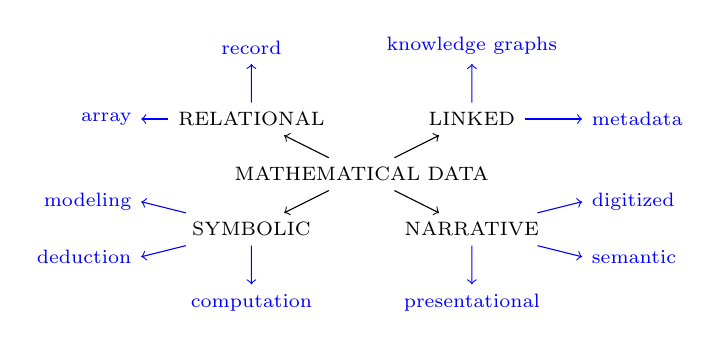
\begin{tikzpicture}
\begin{scope}[font=\scriptsize,scale=.7]
\begin{scope}[]
\node (m) at (0,0) {MATHEMATICAL DATA};
\end{scope}
\begin{scope}[]
\node (s) at (-2,-1) {SYMBOLIC};
\node (r) at (-2,1) {RELATIONAL};
\node (l) at (2,1) {LINKED};
\node (n) at (2,-1) {NARRATIVE};
\draw[->] (m) -- (s);
\draw[->] (m) -- (l);
\draw[->] (m) -- (r);
\draw[->] (m) -- (n);
\end{scope}

\begin{scope}[blue]
\draw[->] (r) -- ++(0,1) node[above] {record};
\draw[->] (r) -- ++(-2,0) node[left] {array};
\draw[->] (l) -- ++(0,1) node[above] {knowledge graphs};
\draw[->] (l) -- ++(2,0) node[right] {metadata};
\draw[->] (s) -- ++(-2,.5) node[left] {modeling};
\draw[->] (s) -- ++(-2,-.5) node[left] {deduction};
\draw[->] (s) -- ++(0,-1) node[below] {computation};
\draw[->] (n) -- ++(2,0.5) node[right] {digitized};
\draw[->] (n) -- ++(2,-.5) node[right] {semantic};
\draw[->] (n) -- ++(0,-1) node[below] {presentational};
\end{scope}
\end{scope}
\end{tikzpicture}
\caption{Kinds of mathematical data}\label{fig:mathematical-data}
\end{figure}

In order to better analyze the current state of the art of FAIRness in mathematical data, we introduce a novel categorization of mathematical data.
An overview is given in Figure~\ref{fig:mathematical-data}.
Each kind of data makes different abstractions or focuses on different aspects of mathematical reality, resulting in characteristic strengths and weaknesses.
We summarize these in Figure~\ref{fig:datakinds}.

\begin{figure}[hbt]\centering\footnotesize
\begin{tabular}{|p{3.5cm}|cccc|}\hline
Kind of data & Sym. & Rel. & Lin. & Nar.\\\hline
Machine-understandable  & \textbf{+} & \textbf{+} & \textbf{+}& \textbf{--}\\
Complete description & \textbf{+} & \textbf{+} & \textbf{--}& \textbf{+}\\
Applicable to all objects & \textbf{+} & \textbf{--} & \textbf{+}& \textbf{+}\\
Easy to produce  & \textbf{--} & \textbf{+} & \textbf{+}& \textbf{+}\\
\hline
\end{tabular}
\caption{Advantages of different kinds of data}\label{fig:datakinds}
\end{figure}

\paragraph*{Symbolic data} consists of formal expressions such as formulas, formal proofs, programs, etc.
These are written in a variety of highly-structured formal languages specifically designed for individual domains and with associated tools.
The most important such domains are \textbf{modeling}, \textbf{deduction}, and \textbf{computation} employing modeling languages, logics, resp. programming languages.
The associated tools like simulation tools, proof assistants, resp. computer algebra systems can understand the entire semantics of the data.

Because symbolic data allows for abstraction principles such as underspecification, quantification, and variable binding, it can capture the complete semantics of any mathematical object.
However, the formalization of a typical narrative theorem as a statement in a proof assistant or a function in a computer algebra system can be very expensive.
This comes at the price of being context-sensitive: expressions cannot be easily moved across environments, which makes \emph{Finding}, \emph{Reusing}, and \emph{Interoperability} difficult.

Moreover, because each tool usually defines its own formal language and because these are usually mutually incompatible, interoperability and reuse across these individual tools are practically non-existent.
To overcome this problem, multiple representation formats have been developed for symbolic data, usually growing out of small research projects and reaching different degrees of standardization, tool support, and user following.
These are usually optimized for specific applications, and little cross-format sharing is possible.
In response to this problematic situation, standard formats have been designed such as MathML~\cite{CarlisleEd:MathML3:on} and OMDoc/MMT~\cite{uniformal:on}.
%The latter has been used as an interoperability format for computer algebra systems in the OpenDreamKit project and already offers comprehensive services for symbolic data such as querying. 

\paragraph{Relational data} employs representation theorems that allow encoding mathematical objects as ground data built from numbers, strings, tuples, lists, etc.
Thus, relational data combines optimized storage and processing with capturing the whole semantics of the objects.
It is also easy to produce and curate as general purpose database technologies and interchange formats such as CSV or JSON are readily available.

Relational datasets can be subdivided based on the structure of the entries, which often enable different optimized database solutions.
The most important ones are record data, where datasets are sets of records conforming to the same schema and which are stored in relational databases, and \textbf{array} data, which consists of very large, multidimensional arrays stored in optimized array databases. %% tree and graph data?
%Array data tends to come up in settings with large but simply-structured datasets such as simulation time series, while record data is often needed to represent complex objects, especially those from pure mathematics.

However, these representation theorems do not always exist because sets and functions, which are the foundation of most mathematics, are inherently hard to represent concretely.
Moreover, the representation theorems may be very difficult to establish and understand, and there may be multiple different representations for the same object.
Therefore, applicability is limited and must be established on a case by case basis.

Therefore, \emph{Interoperability} is difficult because users need to know the exact representation theorem and the exact way how it is applied to understand the encoding.
Therefore, even if the representation function is documented, \emph{Finding}, \emph{Reuse}, and \emph{Interoperability} are theoretically difficult, practically expensive, and error-prone.
For example, consider the following very recent incident from (Jan. 2019): 
There are two encoding formats for directed graphs, both called \texttt{digraph6}: Brendan McKay's \cite{McKayFormats:on} and the one used by the GAP package Digraphs \cite{GAPDigraphFormat:on}, whose authors were unaware of McKay's format and essentially reinvented a similar one \cite{digraph6issue:on}.
The resulting problem has since been resolved but not without causing some misunderstandings first.

\paragraph{Linked data} introduces identifiers for objects and then treats them as blackboxes, only representing the identifier and not the original object.
The internal structure and the semantics of the object remain unspecified except for maintaining a set of named relations and attributions for these identifiers.
This abstraction allows for universal applicability at the price of not representing the complete mathematical object.

The named relations allow forming large networks of objects, and the attributions of concrete values provide limited information about each one.
Linked data can be subdivided into \textbf{knowledge graphs} based on mathematical ontologies and \textbf{metadata}, e.g., as used in publication indexing services.

As linked data forms the backbone of the Semantic Web, linked data formats are very well-standardized: data formats come as RDF, the relations and attributes are expressed as ontologies in OWL2, and RDF-based databases (also called triplestores) can be queried via SPARQL.
For example, services like DBPedia and Yago crawl various aspects of Wikipedia to extract linked data collections and provide SPARQL endpoints.
%They supply a valuable fallback for the linked data ontologies to be developed in the \pn project.
The WikiData database~\cite{wikidata:on} collects such linked data and uses them to answer queries about the objects.
%This makes WikiData a primary target for the purposes of linked data management in \pn. 

Thus, contrary to, linked data has very good FAIR-readiness, in particular allowing for URI-based \emph{Access}, efficient \emph{Finding} via query languages, and URI-mediated \emph{Reuse} and \emph{Interoperability}.
%For example, it is general practice to use the URIs of the respective Wikipedia articles unless more specific ontologies are available.
However, this FAIR-readiness comes at the price of not capturing the complete semantics of the objects so that \emph{Access} and \emph{Finding} are limited and \emph{Interoperability} and \emph{Reuse} are subject to misinterpretation.


\paragraph{Narrative data} consists of mathematical documents and text fragments. We speak of \textbf{mathematical vernacular} for the peculiar mixture of mathematical formulae, natural language with special idioms, and diagrams. There are four levels of formality of narrative data:
\begin{compactenum}
\item \textbf{digitized:} scanned into images from documents,
\item \textbf{presentational:} represented in a form that allows flexible
  presentation on electronic media, such as web browsers;
  born digital or OCRed from digitized ones,
\item \textbf{semantic}: in a form that makes explicit the functional structure and the
  relations between formulae, the objects they denote and the mathematical context.
\end{compactenum}
All levels of formality are relevant for mathematical communication, but machine support for reasoning and knowledge management can only be given at the semantic level.
We could extend this classification by a fourth level of narrative data for formalized documents; but these abstract from the narrative form and are therefore counted as symbolic data.

Note that we can always go from higher levels to lower ones, by styling: presenting semantic features by narrative patterns. Therefore we also count such patterns as narrative data -- e.g. \textbf{notation definitions} such as $\left(n\atop k\right)$ or $\mathcal{C}^n_k$ for the binomial coefficients or verbalizations in different languages.

%%% Local Variables:
%%% mode: latex
%%% mode: visual-line
%%% fill-column: 5000
%%% TeX-master: "report"
%%% End:

%  LocalWords:  centering includegraphics textwidth inparahighlight categorization analyzing summarized ednote hline textbf textbf textbf textbf emph emph emph standardization optimized texttt triplestores LehIseJak:dlsmkbew13 HofSucBer:yago2a analyze formalization digitized calbf verbalizations tikz formalized summarize well-standardized mathcal


\subsection{Deep FAIRness}\label{sec:deep}
 \begin{figure*}[ht]\centering
\begin{tabular}{|l|ll|}
\hline
Service & Shallow & Deep \\
\hline
Identification & DOI for a dataset & DOIs for each entry \\
Provenance & who created the dataset? & how was each entry computed? \\
Validation & is this valid XML? & does this XML represent a set of polynomials? \\
Access & download a dataset & download a specific fragment\\
Finding & find a dataset & find entries with certain properties\\
Reuse & \multicolumn{2}{c|}{impractical without accessible semantics}\\
Interoperability & \multicolumn{2}{c|}{impossible without accessible semantics}\\
\hline
\end{tabular}
\caption{Examples of shallow and deep FAIR services}\label{fig:deepfair}
\end{figure*}
% \ednote{In the table with shallow/deep services the meanings of deep as ``datum level'' and ``mathematical meaning all the way through'' are being mixed}

\begin{figure*}[ht]\centering
  \begin{tabular}{|l||l|l|l|l|}\hline
    Data & Findable & Accessible & Interoperable & Reusable \\\hline\hline
    Symbolic & Hard & Easy & Hard & Hard \\\hline
    Relational & \multicolumn{4}{c|}{Impossible without access to the encoding function} \\\hline
    Linked & \multicolumn{4}{c|}{Easy but only applicable to the small fragment of the semantics that is exposed} \\\hline
    Narrative & Hard & License-encumbered & \multicolumn2{c|}{Human-only}\\\hline
  \end{tabular}
  \caption{Deep FAIR readiness of mathematical data}\label{fig:FAIR-readiness}
\end{figure*}

Relational and linked data can be easily processed and shared using standardized formats such as CSV or RDF.
But in doing so, the semantics of the original mathematical objects is not part of the shared resource: in relational data, understanding the semantics requires knowing the details of the representation theorem and the encoding; in linked data, almost the entire semantics is abstracted away anyway, which also makes it hard to precisely document the semantics of the links.
For datasets with very simple semantics, this can be remedied by attaching informal labels (e.g., column heads for relational data), metadata, or free-text documentation.
But this is not sufficient for datasets in mathematics and related scientific disciplines where the semantics is itself very complex.

For example, an object's semantic type (e.g., ``polynomial with integer coefficients'') is typically very different from the type as which it is encoded and shared (e.g., ``list of integers'').
The latter allows reconstructing the original, but only if its type and encoding function (e.g., ``the entries in the list are the coefficients in order of decreasing degree'') are known.
Already for polynomials, the subtleties make this a problem in practice, e.g., consider different coefficient orders, sparse vs. dense encodings, or multivariate polynomials.
Even worse, it is already a problem for seemingly trivial cases like integers: for example, the various datasets in the LMFDB use at least 3 different encodings for integers (because the trivial encoding of using the CPU's built-in integers does not work because the involved numbers are too big).
But mathematicians routinely use much more complex objects like graphs, surfaces, or algebraic structures.

We speak of \textbf{accessible semantics} if data has metadata annotations that allow recovering the exact semantics of the individual entries of a data set.
Notably, in mathematics, this semantics metadata is very complex, usually symbolic data itself that cannot be easily annotated ad hoc.
But without knowing the semantics, mathematical datasets only allow FAIR services that operate on the dataset as a whole, which we call \textbf{shallow} FAIR services.
But it is much more important to users to have \textbf{deep} services, i.e., services that process individual entries of the dataset.

Figure~\ref{fig:deepfair} gives some examples of the contrast between shallow and deep services.
Note that deep services do not always require accessible semantics for every entry, e.g., deep accessibility can be realized without.
But many deep services are only possible if the service can access and understand the semantics of each entry of the dataset, e.g., deep search requires checking for each entry whether it matches the search criteria.

In mathematics, shallow FAIR services are relatively easy to build but have significantly smaller practical relevance than deep FAIR services.
Deep services, on the other hand, are so difficult to build that they are essentially non-existent except when built ad hoc for individual datasets.
Figure~\ref{fig:FAIR-readiness} gives an overview of the difficulty for the different kinds of data.


Note that deep FAIR services are particularly desirable in mathematics, their advantages are by no means limited to mathematics.
For example, in 2016 \cite{ZieEreElO:GeneErrors16}, researchers found widespread errors in papers in genomics journals with supplementary Microsoft Excel gene lists. 
About 20\% of them contain erroneous gene name because the software misinterpreted string-encoded genes as months.
In engineering, encoding mistakes can quickly become safety-critical, i.e., if a dataset of numbers is shared without their physical units, precision, and measurement type.
With accessible semantics, datasets can be validated automatically against their semantic type to avoid errors such as falsely interpreting a measurement in inch as a measurement in meters, a gene name as a month, or a column-vector matrix as a row-vector matrix.

%We aim to build a coherent representation standard for mathematical data that systematically makes the semantics accessible.
%This enables (i) prototyping universally applicable Deep FAIR services that improve on the existing ad hoc or limited solutions and (ii) making a wide variety of existing datasets available via a central platform.

In order to support the development Deep FAIR services for mathematics, we extend the original FAIR requirements from~\cite{WilDumAal:FAIR16}, which focused on shallow FAIR, to deep FAIR:
\begin{enumerate}
  \item[\textbf{DF}] The internal structure of each object is represented and indexed in a way that allows searching for individual entries.
  \item[\textbf{DA}] Each dataset includes a representation of the semantics of the represented objects.
  %representation of each object semantics stays accessible even after the objects are no longer available.
  \item[\textbf{DI}] The representation of each object uses a formal, accessible, shared, and broadly applicable language for knowledge representation, uses FAIRly shared vocabularies, and where applicable includes qualified references to other representations.
  \item[\textbf{DR}] The representation of each object is richly described with a plurality of accurate and relevant attributes, is released with a clear and accessible data usage license, is associated with detailed provenance information, and meets domain-relevant community standards.
\end{enumerate}

%%% Local Variables:
%%% mode: latex
%%% mode: visual-line
%%% fill-column: 5000
%%% TeX-master: "report"
%%% End:

%  LocalWords:  textbf inparahighlight centering hline bigskip newpart textwidth textwidth OAFproject:on Modelica Modelica:on ConderCensuses:on LeemansPolytopes:on PotocnikCensuses:on cdot10 cdot lmfdb:on zbMATH zbMATH:on disambig swMATH swMATH:on ednote realized standardized


\subsection{MathDataHub}\label{sec:hub}
 We present a unified infrastructure to support Deep FAIR for relational mathematical data.
It builds on our MathHub system, a portal for narrative and symbolic mathematical data.
MathDataHub is a part of the MathHub portal and provides storage and hosting with integrated support for Deep FAIR.
In the future, this will also allow for the development of mathematical query languages (i.e., queries that abstract from the encoding) and mathematical validation (e.g., type-checking relative to the mathematical types, not the database types).

The Workshop on Mathematical data in Cernay, France (August 17-24th),
was dedicated to improving the status of relational data in mathematics.
The workshop brought together interested users and authors of mathematical datasets, 
data framework developers, 
and experts interested in integrating mathematical databases with computer algebra systems.
The workshop enabled progress on several fronts.
We sketched out a submission and editorial process for the platform.
We also imported several real-life datasets into the system.

\paragraph{Census of relational data in mathematics}
In some areas of mathematics, research products can consist of
listings or tabulations of complex mathematical objects and their properties.
These datasets can be later used by researchers to form or refute conjectures.
To facilitate the collection of information about relational data in mathematics,
we set up a database with a website frontend~\cite{bercic:cmo:table}.
While it grew out of the necessity to keep track of the information, 
it has at least two further goals.
First, it aims to make it easy for anyone to see what information has been collected so far.
Second, it aims to eventually make it easy to contribute information.

The information about the datasets can be displayed a few different views
(with switching implemented through tabs): 
general information, information about size, 
information pertaining to the FAIR principles,
as well as some other properties.

Currently, the census contains about $70$ datasets from several areas of mathematics.
This includes links to dataset websites and author information for (nearly) all of the datasets,
as well as literature references, area of mathematics and size-related information for many.
Even this small sample shows large variations in terms of
structure, content organisation, provenance, infrastructure and shareability, and size.

Perhaps the most important immediate use for this census is as a 
``market study'' for MathDataHub.
It serves as a source of use cases for the infrastructure,
as well as beginnings of a community of researchers that work with mathematical data.
Even in this initial stage, the census gives the developers of MathDataHub
some idea of the requirements for the system in terms of the ranges of
dataset size, complexity, etc.

We will continue to gather information about the relational datasets 
in mathematics in the living census website.
Finally, we plan to use the new information as a basis for a more structured census.

\paragraph{Mathematical data description language (MDDL)}
We developed a mathematical data description language MDDL in~\cite{BerKohRab:tumdi19} (Math Data Description Language) that uses symbolic data to specify the semantics of relational data.
MDDL schemas combine the low-level schemas of relational database with high-level descriptions (which critically use symbolic mathematical data) of the mathematical types of the data in the tables.

\begin{figure}[ht]
  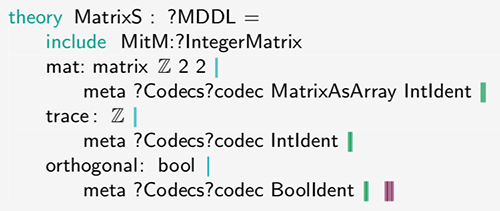
\includegraphics[width=.48\textwidth]{data_joe-schema}
  \caption{Schema theory for Joe's dataset}\label{fig:joe-schema}
\end{figure}

To fortify our intuition let us assume that Joe has collected a set of integer matrices together with their trace
and the Boolean property whether they are orthogonal.
Figure~\ref{fig:joe-schema} shows a MDDL theory that describes his database schema.
For example, the mathematical type of the field $\mathsf{mat}$ is integer $2\times2$ matrices;
the $\mathsf{codec}$ annotation specifies how this mathematical type is be encoded as a low-level database type (in this case: arrays of integers).
Concretely, the codec is $\mathsf{MatrixAsArray}$ codec operator applied to the identity codec for integers.
These codec annotations capture the representation theorem that allows representing the mathematical objects as ground data that can be stored in databases. 
%The tag \textsf{opaque} specifies that matrices cannot be used for filtering in the user interface. 

The information is sufficient to generate a database schema -- here one table with columns $\mathsf{mat}$, $\mathsf{trace}$, and $\mathsf{orthogonal}$ -- as well as a database browser-like website frontend (see Figure~\ref{fig:joe}).
The generation of APIs for computational software such as computer algebra systems is also possible and currently under development. 

\begin{figure}[ht]
  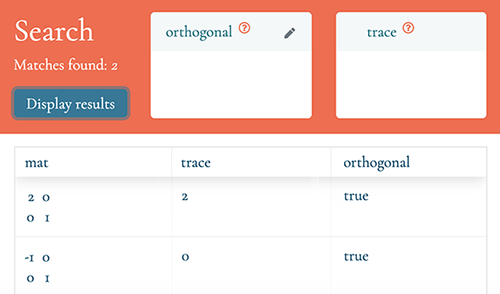
\includegraphics{data_joe.png}
  \caption{Website for Joe's dataset}\label{fig:joe}
\end{figure}

Crucially,  the codec-based setup transparently connects the mathematical level of specification with the database level -- a critical prerequisite for the deep FAIR properties postulated above.
Moreover, in Figure~\ref{fig:joe-schema}, the mathematical background knowledge is imported from a theory $\mathsf{IntegerMatrix}$ in the Math In The Middle ontology (MitM)~\cite{MitM:on}, which supplies the full mathematical specification and thus the basis for \emph{Interoperability} and \emph{Reusability}; see~\cite{BerKohRab:tumdi19,WieKohRab:vtuimkb17,KohMuePfe:kbimss17} for details.
The overhead of having to specify the semantics of the mathematical data is offset by the fact that we can reuse central resources like the MitM ontology and codec collection. 
Thus, MitM and MDDL form the nucleus of a common vocabulary for typical mathematical relational datasets. 
%These can and should eventually be linked to representation standards in other domains. 
%For mathematical datasets, the math-specific aspects attacked by our work are the dominant factor.

\paragraph{Web-Interface Analysis}
At the Workshop on Mathematical Data,
Andrea Kohlhase tested the user experience of the existing web interface
through user interviews.
The list of issues identified through the interviews is available at the 
workshop repository\footnote{https://github.com/OpenDreamKit/MathDataWorkshop/issues/3}.
Andrea Kohlhase also produced a clickable prototype of an updated interface
and used that in a few interviews combined with an eye-tracker test.




%%% Local Variables:
%%% mode: latex
%%% mode: visual-line
%%% fill-column: 5000
%%% TeX-master: "report"
%%% End:

%  LocalWords:  flexiformal BerKohRab:tumdi19 includegraphics textwidth textbf textsf textsf textsf ednote BerKohRab:tumdi19,WieKohRab:vtuimkb17,KohMuePfe:kbimss17 externalize Cernay shareability mathsf emph emph

%%% Local Variables:
%%% mode: latex
%%% mode: visual-line
%%% fill-column: 5000
%%% TeX-master: "report"
%%% End:


\newpage
\section{Semantic Search For Computational Documents}\label{sec:software}
\def\MWS{MathWebSearch\xspace}

In the \pn VRE toolkit approach, a virtual research environment (VRE) is based on software and data components (called D/K/S-bases in the original proposal) under a joint user interface.
Here we concentrate on a crucial aspect of this, the interaction of the D/K/S-base with the UI in mathematical Jupyter notebooks and interactive mathematical documents -- see ~\cite{ODK-D4.2} for a discussion of the concepts.
In particular, mathematical Notebooks allow users to navigate the combined information space of all the underlying tools, systems and
resources integrated into the VRE as one. 
However, they aggravate the already serious problem of finding the piece of knowledge (or Notebook) a mathematician wants.
Of course, there is a text search engine built into  GitHub that can distinguish notebooks by file type, but as well well know, this only helps it the mathematician can already express her information through a bag of words.
When it comes to formulae, the GitHub search engines is essentially blind. 
Thus, we decided to adapt the \MWS formula search engine to this \pn joint user interface. 

\subsection{The \MWS Formula Search Engine}

\MWS is a web application that provides low-latency answers to full-text queries which consist of keywords and formulae.
We give only a brief overview of the pre-existing \MWS architecture here and refer the reader to~\cite{ProKoh:mwssofse12} and ~\cite{ODK-D6.1}. 
We furthermore describe our re-worked design in Section~\ref{sec:software:deployment} below.
In a nutshell, \MWS consists of a search web application (the \MWS daemon) that indexes formula harvests (essentially lists of content MathML formulae and URI references) and answers queries (Content MathML schemata with query variables).
Multiple domain-specific front-ends can talk to the \MWS daemon using an XML-based protocol, they transform the user's information into Content MathML queries. 

The \MWS system has been used to supply search instances on various corpora of mathematical documents, we describe two here, others can be seen on \url{http://search.mathweb.org}. 

\subsubsection{arXiv search}

Begun on August 14, 1991, created by Paul Ginsparg, the ``Cornell e-Print arXiv'' (\url{http://arXiv.org}) is a repository of scientific papers and electronic preprints in
fields of mathematics, computer science, physics, astronomy, biology and statistics or finance written in {\TeX/\LaTeX} for an optimized transfer over the internet and an easily rendered client-side.
In present the project is hosted by Cornell University and includes over a million articles and increases with around 8000 per month.

The KWARC group have converted by arXiv corpus into HTML5~\cite{StaKoh:tlcspx10} and harvested it for \MWS. The instance at \url{http://arxivsearch.mathweb.org}
indexes over 105\,000 math-heavy papers.
This subcorpus has also been used for the NTCIR Math Information Retrieval Challenges~\cite{AizKohOun:nmpto13,AizKohOunSch:nmto14,AizKohOunSch:nmto16}.

\subsubsection{zbMATH search}

Zentralblatt Math (zbMath) is a mathematical information service that curates a database of reviews and classifications (MSC, see~\cite{MSC2010}) for all articles in mathematics since the middle of the 19th century. The database currently contains 3.8 million reviews and grows at a rate of ca 120\,000 reviews per year.
The zbMATH portal at \url{https://zbmath.org/} offers a faceted search engine for reviews based on bibliographic metadata, MSC classification, and \emph{formulae}.
The latter is driven by \MWS. 

\subsection{Enabling Formula Search Deployments}\label{sec:software:deployment}

The previous \MWS deployments required a significant amount of application-specific code. 
This code was typically written by students, and as a result it was not of high quality. 
In particular, most code was too specialized to be re-usable. 

This made it impossible to directly use \MWS inside OpenDreamKit. 
To allow using \MWS flexibly, we needed to inject the system with a lot of software engineering. 
To achieve this, we developed new infrastructure on top of the core \MWS daemon. 
This works takes the form of several components, each of which can deployed independently using Docker (see also \WPref{component-architecture}).
The structure of our infrastructure can be seen in Figure~\ref{fig:mwsdeployment}, with new components in green. 

\begin{figure}[ht]
  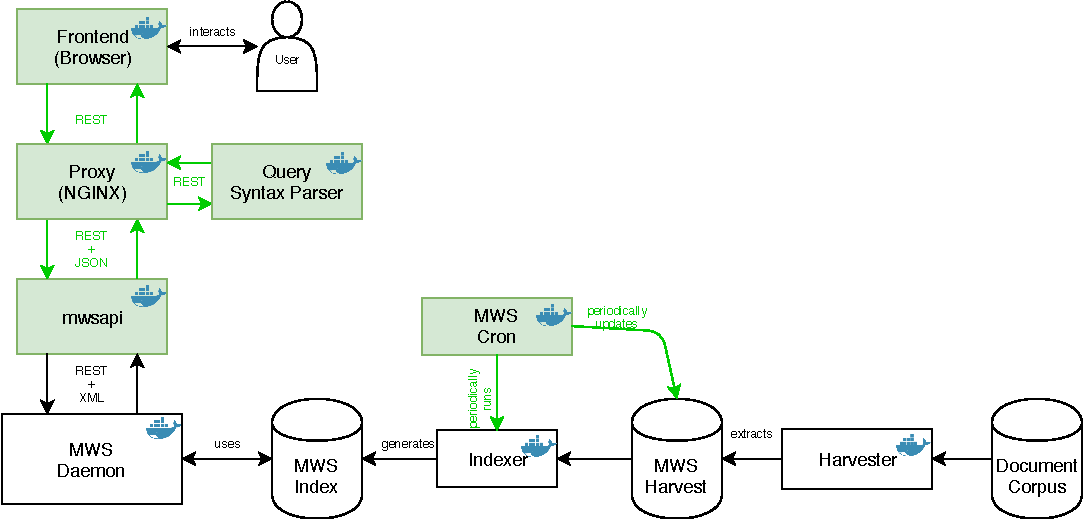
\includegraphics[width=0.8\textwidth]{mws_layout.pdf}
  \caption{Structure of our newly developed \MWS Deployment Infrastructure. Newly developed and updated components colored in green. }\label{fig:mwsdeployment}
\end{figure}

We describe the components of our infrastructure. 

\paragraph{The \MWS Daemon}
The central component is the \textit{\MWS daemon}, which can be found in the bottom left. 
As previously, it uses an \textit{Index} and exposes an XML-based API for queries. 
The only change we made to the core daemon is that it now exists inside a Docker Container at \footnote{\url{https://hub.docker.com/r/mathwebsearch/mathwebsearch/}}. 

\paragraph{The Harvesters and The Indexer}
As before, in order to generate an index from a set of documents we need two components. 
The indexer, as an application-independent component, has also been dockerized \footnote{\url{https://github.com/MathWebSearch/mws-indexer}}. 
First we extract a set of ContentMathML formulae using a corpus-specific \textit{Harvester} (bottom right). 
The generated \textit{Harvest} is then sent to the \textit{Indexer} (bottom center), which generates or updates the \textit{Index}. 

Additionally, we introduced a new scheduler component called \textit{MWS cron}. 
This periodically sends updated harvests to the \textit{indexer}, which then in turn updates the index. 
This process ensures that the Index remains up-to-date, and does not have to be re-generated manually. 
The source code of this component can be found at \footnote{\url{https://github.com/MathWebSearch/mws-cron}}. 

\paragraph{Frontend, mwsapi and the query syntax parser}

In order to process end user queries, we introduced several additional components.

The most important component of these is a new React-powered \textit{frontend}\footnote{\url{https://github.com/MathWebSearch/frontend}}, which runs inside the users' browser. 
It allows users to enter a formula search query, and view the results. 
The frontend contains corpus-specific branding and text, and is otherwise not corpus-specific. 
In particular the querying code which interacts with the backend components, does not require specialization. 

While the \MWS daemon only understands formulae in Content MathML, users often enter them using different representations, such as \LaTeX. 
For this purpose, the frontend allows entering queries in human-writable, corpus-specific syntax. 
In order to transform the user query into a system-understood query, we make use of a new component called the \textit{Query Syntax Parser}. 
For {\LaTeX} syntax this is achieved using {\LaTeX}ML along with a custom \MWS extension, but this component is fully interchangeable if the user desires other syntaxes. 

The frontend does not directly send MathML queries to the \textit{Daemon}.
Instead, it sends them to a thin API layer on top called \textit{mwsapi}. 
This layer forwards the queries to the daemon and, upon receiving a response, performs some post-processing. 
This process includes transforming substitutions returned by \MWS into a format that can be directly presented to the user by the frontend. 
The layer is written in go and doubles as api bindings to use MathWebSearch programatically in other applications. 
The source code and documentation are available on Github at \footnote{\url{https://github.com/MathWebSearch/mwsapi}}. 

As the frontend, the mwsapi server and the Query Syntax Presenter are all exposed to the end-user under the same url, a proxy delegating requests accordingly was also necessary. 
This is using an nginx server. 

\subsection{Building a Notebook Search}

Sage can produce \LaTeX\ formulae as output\ednote{TW@MK: Not sure how to describe this in more detail; should we ask Nicolas for this?}.
Using the newly developed infrastructure above, it was straightforward to apply \MWS and enable users to search for these formulae. 

Applying our infrastructure involved two steps, which we briefly describe below.

\paragraph{Harvesting Formulae}
To enable \MWS to search the formulae, we needed to build a harvester that extracted formulae from a notebook and as ContentMathML formulae. 
To achieve this, we converted each \LaTeX\ formula via LaTeXML and aggregated them inside an \MWS Harvest file. 
The script to achieve this can be found at \footnote{\url{https://github.com/OpenDreamKit/jupyter-notebook-harvester/blob/master/harvest}} and involved around 100 lines of straightforward Python script written in a few hours. 

To test our harvester, we decided to make use of Sage Jupyter Notebooks found on GitHub. 
We implemented a second Python script which used the GitHub API to download all matching files and then apply our harvester to them. 
This process resulted in an \MWS Harvest of $0$ documents, containing $0$ formulae\ednote{TW: Update numbers}.

\paragraph{Query Syntax Parser}

To enable users to search the formulae in an appropriate syntax, a query syntax parser was required. 
However, as Sage produces \LaTeX\ formulae, we can re-use the {\LaTeX}ML query syntax parser for this purpose. 

\paragraph{Deploying the system}

\begin{figure}[ht]
  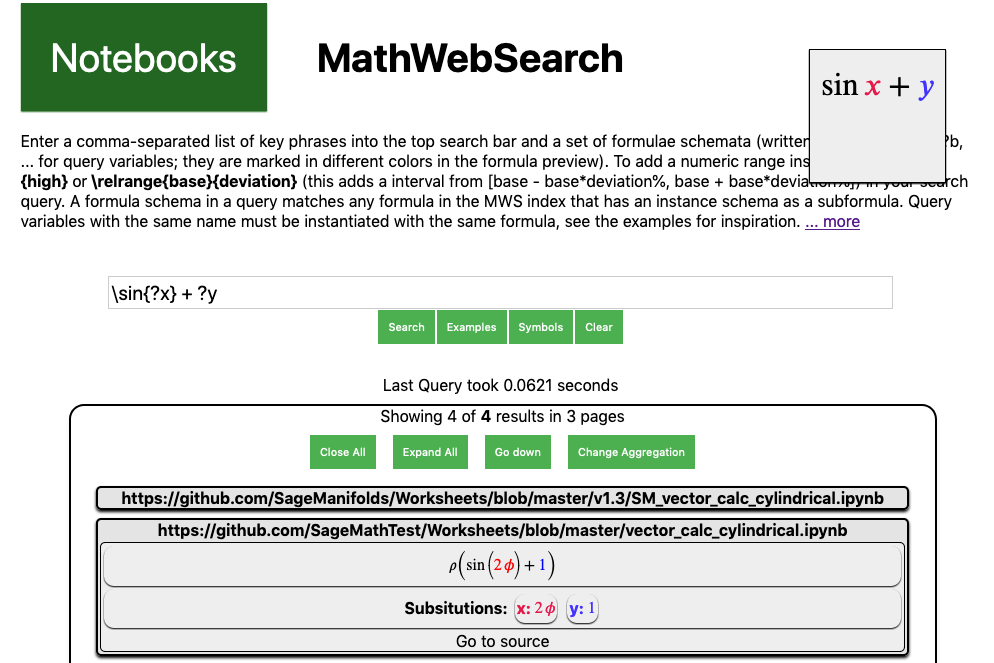
\includegraphics[width=\textwidth]{mwsnotebookfront.png}
  \caption{The deployed Jupyter Notebook Search Frontend}\label{fig:mwsnotebookfront}
\end{figure}

The third and final step involved deploying the system.
This required minor customization in the branding of the frontend. 
The user interface is deployed at \url{https://jupytersearch.mathweb.org} and can be seen in Figure~\ref{fig:mwsnotebookfront}.

In addition the notebook search, we have also exercised a similar progress for the $n$-category Cafe (nLab, \url{https://ncatlab.org/}, a community-run semantic wiki on category theory and applications with more than 13K pages). 
Similar to notebooks, NLab also contains formulae in \LaTeX\ syntax, enabling us to largely re-use all components we had created previously.  The NLab Harvester can be found at \footnote{\url{https://github.com/MathWebSearch/nlab_harvester}}, and the corresponding frontend at \url{https://nlabsearch.mathweb.org}.

%%% Local Variables:
%%% mode: latex
%%% mode: visual-line
%%% fill-column: 5000
%%% TeX-master: "report"
%%% End:

%  LocalWords:  ednote textbf fig:mwsdeployment includegraphics textwidth mws_layout.pdf textit mwsapi specialization nginx Jupyter customized evalutation temasearch xspace newpart standardized ProKoh:mwssofse12 subsubsection Ginsparg optimized StaKoh:tlcspx10 AizKohOun:nmpto13,AizKohOunSch:nmto14,AizKohOunSch:nmto16 zbMATH emph specialized WPref colored dockerized customization NLab oldpart mwsnotebookfront.png fig:mwsnotebookfront


\newpage
\section{Conclusion}
The main achievements made in Work Package 6 over the last year of the OpenDreamKit project were:
\begin{compactenum}
\item the re-conceptualization of integrating the different aspects of doing mathematics, which led to a better understanding of the nature and intended semantics of VRE components (see Section~\ref{sec:tetrapod}),
\item the integration of a major formal knowledge base into the MitM Ontology, which provides the pivotal point for system integration and service discovery (see Section~\ref{sec:knowledge}),
\item the development of a semantic model for mathematical datasets (see Section~\ref{sec:data}), which has been used in \WPref{dksbases} in two ways: 
  \begin{compactitem}
  \item The Warwick group inventoried all the LFMDB datasets, and to (manually) recover their specifications (schema information) at the mathematical and data base level.
    In essence this retrofits the existing LFMDB project with the a more semantic level and has led to a vastly improved and more semantic API for LMFDB (see \url{http://www.lmfdb.org/api2/}) that has recently come online.
    Moreover, a \Sage interface based on this new API is currently under development.
  \item The Erlangen group built a from-scratch implementation of a hub for mathematical data (see Section~\ref{sec:hub}).
  \end{compactitem}
\item special and adapted search facilities for all kinds of mathematical data and VRE components (see Section~\ref{sec:software}),
\item a standalone implementation of persistent memoization in Python and GAP (see \delivref{dksbases}{persistent-memoization}).
\end{compactenum}
Several of these were described in detail in this report.
In order to describe the general picture, we briefly go over the various parts in the rest of this section.

\paragraph{Knowledge}
We have introduced an upper ontology for formal mathematical libraries (ULO), which we propose as a community standard, and we exemplified its usefulness at a large scale.
We posit ULO as an interface layer that enables a separation of concerns between library maintainers and users/application developers.
Regarding the former, we have shown how ULO data can be extracted from formal knowledge libraries such as Isabelle.
We encourage other library maintainers to build similar extractors.
Regarding the latter, we have shown how powerful, scalable applications like querying can be built with relative ease on top of ULO datasets.
We encourage other users and library-near developers to build similar ULO applications, or using future datasets provided for other libraries.

Finally, we expect our own and other researchers' applications to generate feedback on the specific design of ULO, most likely identifying various omissions and ambiguities.
We will collect these and make them available for a future release of ULO 1.0, which should culminate in a standardization process.

\paragraph{Data}
We have analyzed the state of research data in mathematics with a focus on the instantiation of the general FAIR principles to mathematical data.
Realizing FAIR mathematical data is much more difficult than for other disciplines because mathematical data is inherently complex, so much so that datasets can only be understood (both by humans or machines) if their semantics is not only evident but itself suitable for automated processing.
Thus, the accessibility of the mathematical meaning of the data in all its depth becomes a prerequisite to any strong infrastructure for FAIR mathematical data.

Based on these observations, we developed the concept of Deep FAIR research data in mathematics.
As a first step towards developing a Deep FAIR--enabling standard for mathematical datasets, we focused on relational datasets.
We presented the prototypical \dmh system, which lets mathematicians integrate a dataset by specifying its semantics using a central knowledge and codec collection.
We expect that \dmh also helps alleviate the problem of \emph{disappearing datasets}:
Many datasets are created in the scope of small, underfunded or unfunded research projects, often by junior researchers or PhD students, and are often abandoned when developer change research areas or pursue a non-academic career.

\paragraph{Software: computational mathematical documents}
For the S aspect of what was called D/K/S-structures in the \pn proposal or the \textbf{narration} and \textbf{computation} aspects of the finer tetrapod model from Figure~\ref{fig:tetrapod}, we have developed a formula harvester for Jupyter notebooks and a formula search engine that builds on them.

To make this possible, we had to invest a heavy dose of software engineering into the MathWebSearch system: Even though the system has successfully been used as a formula search engine in the zbMATH publication information system (see \url{https://zbmath.org/formulae/}), the deployment of the system required a lot of domain-specific development and workflow integration.
To this end we have developed Go bindings for the MathWebSearch daemon, documented the interfaces, and provided a web application wrapper.
With this, specific applications only need a domain-specific harvester and minimal customization of our generic front-end. 
We have exercised that for the Jupyter Search engine (as envisioned in task \taskref{dksbases}{mws}) and analogously for a formula search engine for the $n$-category Cafe (nLab, see \url{https://nlabsearch.mathweb.org/}).


\paragraph{Persistent Memoization}
As an integration layer between computation and data, we have developed a persistent memoization infrastructure.
Even though it is called ``persistent'' memoization, the temporal scope of the memoized data is potentially less than the eternity-scope of datasets in LMFDB and \dmh.
Indeed, the characteristic innovation in \delivref{dksbases}{persistent-memoization} is that mathematical objects and data can be shared across multiple computations, in multiple systems of in different runs of the same system.
It allows omitting the semantic level, in which case systems are required to ensure data is read in with the same meaning that it had when it was written out.
But it is flexible enough to use \dmh, or a variant of it, as the physical storage of the data.
Thus, the borders between persistent memoization and mathematical datasets become fluent: indeed, datasets often start as private computation caches and gradually become complete, curated, published datasets.
We will study the spectrum and conversions from memoization caches to \dmh datasets in the future. 

%%% Local Variables:
%%% mode: latex
%%% mode: visual-line
%%% fill-column: 5000
%%% TeX-master: "report"
%%% End:

%  LocalWords:  standardization analyzed Realizing emph ednote summarizes re-conceptualization WPref dksbases compactitem dmh delivref textbf textbf Jupyter zbMATH taskref mws customization


\newpage
\printbibliography
\end{document}

%%% Local Variables:
%%% mode: latex
%%% mode: visual-line
%%% fill-column: 5000
%%% TeX-master: t
%%% End:

%  LocalWords:  github githubissuedescription ednote subsubsections newpage tableofcontents Formalized conc printbibliography maketitle
